%!TEX root = ../Thesis.tex
% \pagebreak[4]
\chapter{Correlation for Adaptively Focused Imaging}\label{chap:CAFI}

\graphicspath{{CAFI/Images/}{CAFI/Images/EPS/}{CAFI/Images/Results/}}

\section{Introduction}
Spatially Averaged Sub-Aperture Correlation Imaging (SASACI), described in Chapter \ref{chap:SASACI}, has shown potential in reducing noise caused by large grains\cite{lardner_new_2013} but this technique has a number of limitations. The first is due to the need for a range of input variables. Hence, the resulting output image is sensitive to the parameter settings and these parameters require a degree of trial and error in order to select the values that will give optimal results for a given inspection scenario. The second major limitation is resolution. While speckle noise is reduced, resolution is decreased, preventing characterization of any genuine flaws.

A new technique, Correlation for Adaptively Focused Imaging (CAFI), is now proposed which builds upon the SASACI technique\cite{lardner_using_2014}. This technique aims to solve the problem of generating images of materials with variable propagation velocities, while not being sensitive to parameter settings. CAFI is inspired by the Nearest Neighbour Cross-Correlation (NNCC) technique, introduced by Flax \& O'Donnell in 1988\cite{flax_phase-aberration_1988}.


\section{Methodology}
Correlation for Adaptively Focused Imaging (CAFI) processes FMC datasets to create images in the same manner as TFM and SASACI, but utilizes cross-correlation to improve focusing in materials where there are local velocity variations. It does this by amending the delays applied to each element so that the cross-correlation coefficient of neighbouring signals are maximised.

A flowchart outlining the cross-correlation methodology for CAFI is shown in Figure \ref{fig:cafi_flowchart}. The technique processes each transmitting element and pixel individually and each iteration of the loop is referred to as a TxPx. First, for each receive element, the estimated delay (for delay-and-sum imaging) is calculated. A range of samples is then extracted from the A-scan centred on the calculated delay. Once this has been completed for every receiving element for a given TxPx combination, the contributions from neighbouring receiving elements are cross-correlated using the equation shown in Equation \ref{eq:cafi_xcorr}, where $C$ is the centre of the signal to be cross-correlated, $S$ is the number of pixels on each side of $C$ to be analysed and $RX1$ and $RX2$ are the signals to be cross-correlated\cite{seo_sidelobe_2008}. The cross-correlation is performed at a range of delays, known as lags, for every pair of receiving elements. The aim of this stage is to find the number of lags, $d$, that results in the highest value of cross-correlation coefficient, $p$. This value is recorded for each pair of adjacent elements. The original delay adjusted by the calculated lags will result in the optimal focus for each TxPx. The corrected delays for a single TxPx are normalized to the centre element so that imaging can take place using the corrected delays. 

\begin{figure}[hp]
\centering
		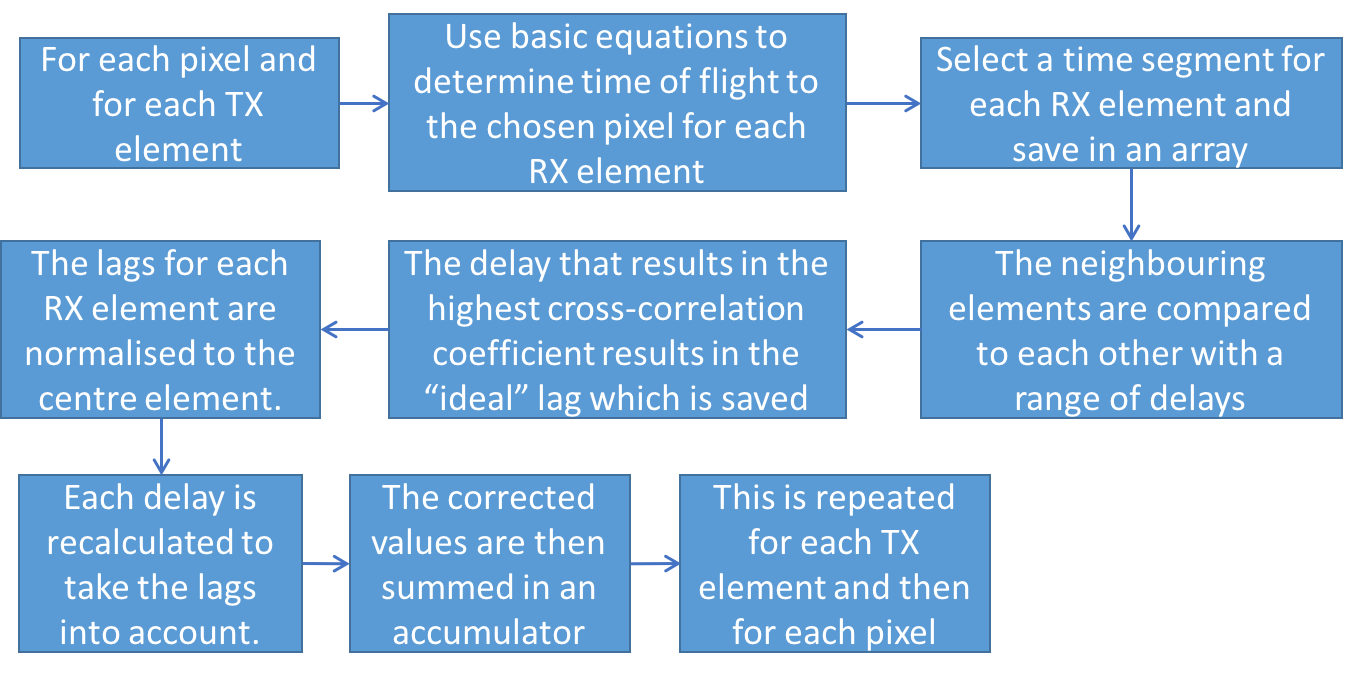
\includegraphics[width=\textwidth]{CAFI_Methodology2.png}
		\caption{The flowchart depicting the cross-correlation process of Correlation for Adaptively Focused Imaging}
		\label{fig:cafi_flowchart}
\end{figure}

 \begin{equation} \label{eq:cafi_xcorr}
p(x) = \frac{\sum\limits_{i = x - S}^{x+S}  RX1(i) \cdot RX2(i-d) }{\sqrt{\sum\limits_{i = x - S}^{x+S} RX1(i)^2} \cdot \sqrt{\sum\limits_{i = x - S}^{x+S} RX2(i-d)^2}}
 \end{equation}

Equation \ref{eq:cafi_xcorr} is repeated for different values of $d$. $d$ is typically set to a range of integers, centred around 0, that relate to the number of samples per wavelength in the signal. Once $d$ has been calculated for each pair of elements within a TxPx combination, the lags are normalised to the centre element using Equation \ref{eq:cafi_D} where $n_{el}$ is the number of array elements. This equation is valid only for the second half of the array, and must be repeated iterating from the centre element towards the first in order to calculate $D$ for the first half of the array.

\begin{equation} \label{eq:cafi_D}
D_{rx} = \sum\limits_{x=\frac{n_{el}}{2}}^{rx-1} d_x - d_{x+1}
 \end{equation}

 \begin{equation} \label{eq:cafi_TFM}
TFM_{TxPx} = | \sum h_{tx,rx} (\frac{\sqrt{(y_{tx} - y)^2 + z^2} + \sqrt{(y_{rx} - y)^2 + z^2}}{v_L} - D_{rx}) |
 \end{equation}

The modified TFM algorithm is shown in Equation \ref{eq:cafi_TFM} where $h_{tx,rx}$ is the FMC matrix, $y_{tx}$ is the location of the transmitting element, $y_{rx}$ is the location of the receiving element, $y$ and $z$ are the co-ordinates of the pixel of interest, $v_L$ is the propagation velocity in the inspection medium, and $D_{rx}$ is the delay adjustment calculated through cross-correlation. The delay adjustment is unique for each transmit-receive pair. $tx$ is constant for Equation \ref{eq:cafi_TFM} and the process is repeated for every TxPx.


\subsection{An Introduction to Nearest Neighbour Cross-Correlation}

To examine how Nearest Neighbour Cross-Correlation (NNCC) works, a simple problem with a transmitter and two receivers is considered. A point reflector in a perfect medium is modelled and it is assumed that there is no energy loss due to absorption or dispersion. The diagram for this model is shown in Figure \ref{fig:cafi_experiment}. A hypothetical scenario will be explored using this model and examine methodologies of combining the responses from the receivers.

\begin{figure}[htbp]
\centering
		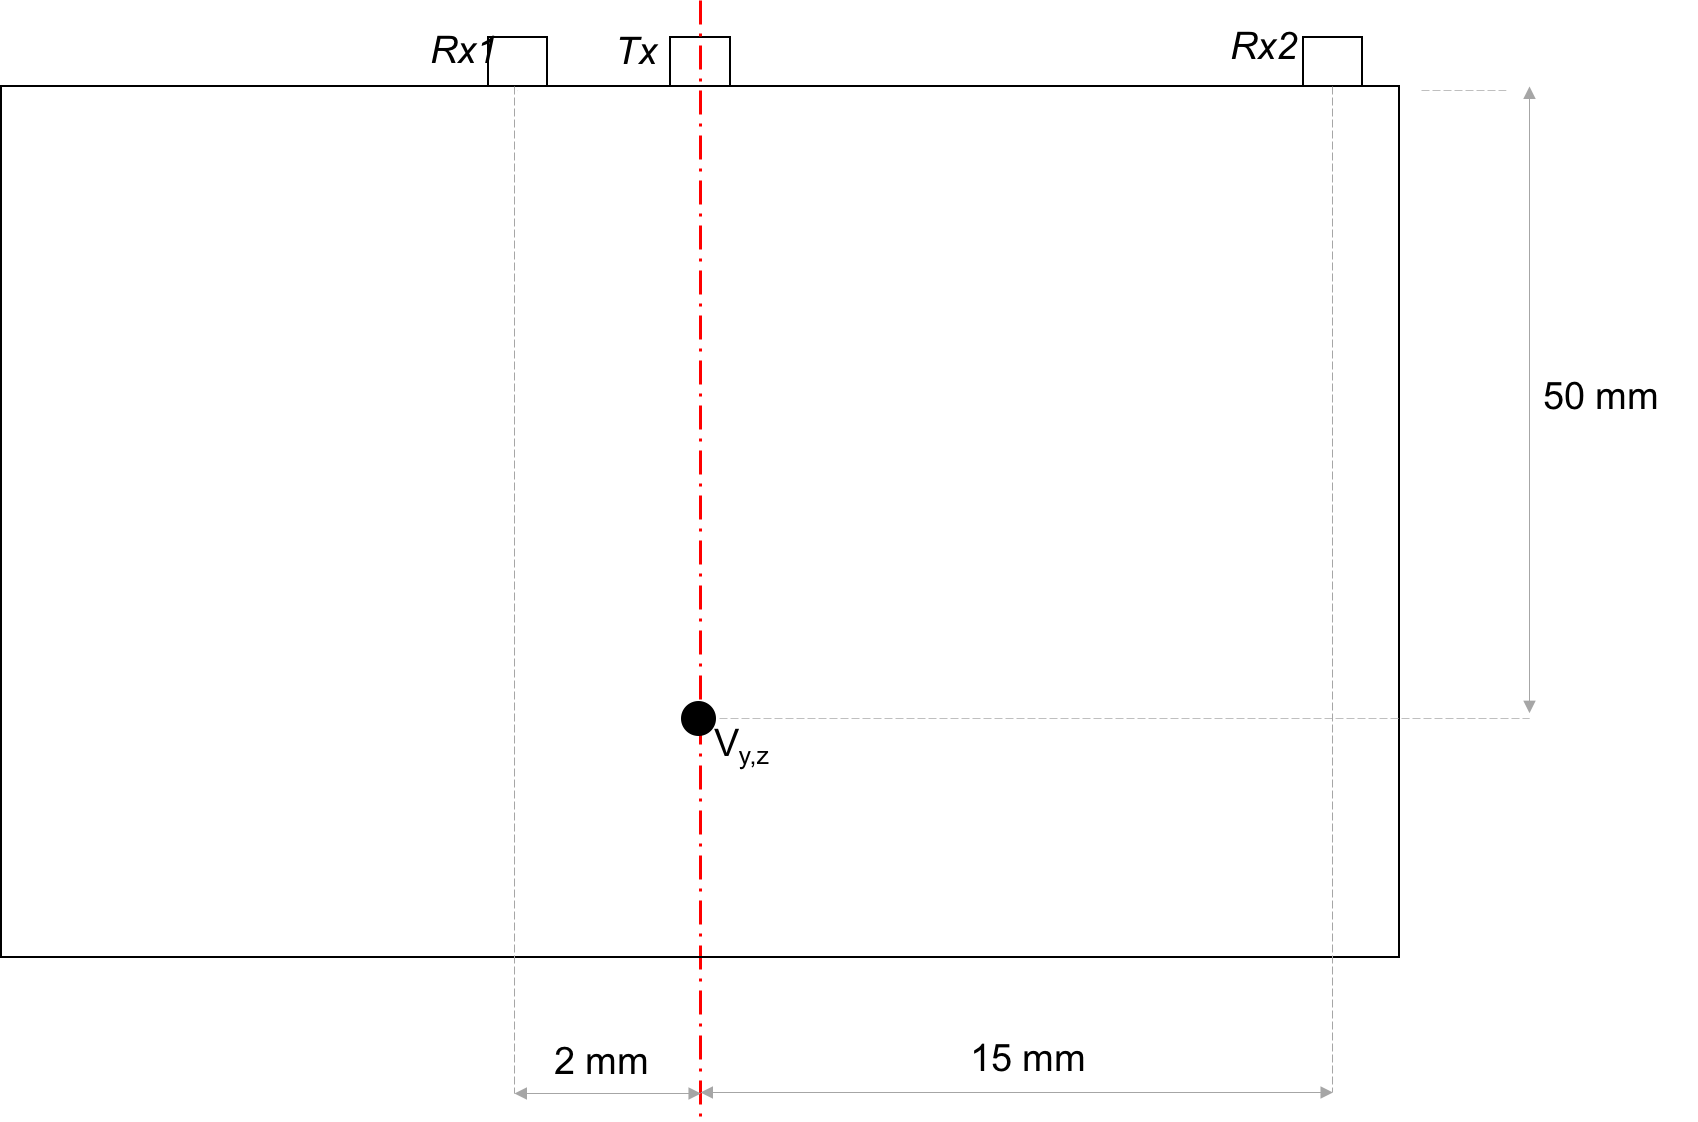
\includegraphics[width=\textwidth]{Experiment3.png}
		\caption{An hypothetical setup with a transmitter, two receivers and a point reflector. Not to scale.}
		\label{fig:cafi_experiment}
\end{figure}

For reference in this chapter, the leftmost receiving element will be referred to as $Rx1$ and the rightmost, $Rx2$. For equations \ref{eq:cafi_delays_general1} to \ref{eq:cafi_delays} a general solution will be sought, referring to any receiving element only as $r_{x,y}$. When a signal is referred to as being combined, it is the summation of the responses from $Rx1$ and $Rx2$.

The input to the system is a Gaussian windowed tone-burst. There are 5 cycles of a 1MHz sine wave, sampled at a frequency of 20MHz and weighted using a standard Gaussian window generated via MATLAB. This is shown in Figure \ref{fig:cafi_toneburst}.

\begin{figure}[htb]
\centering
		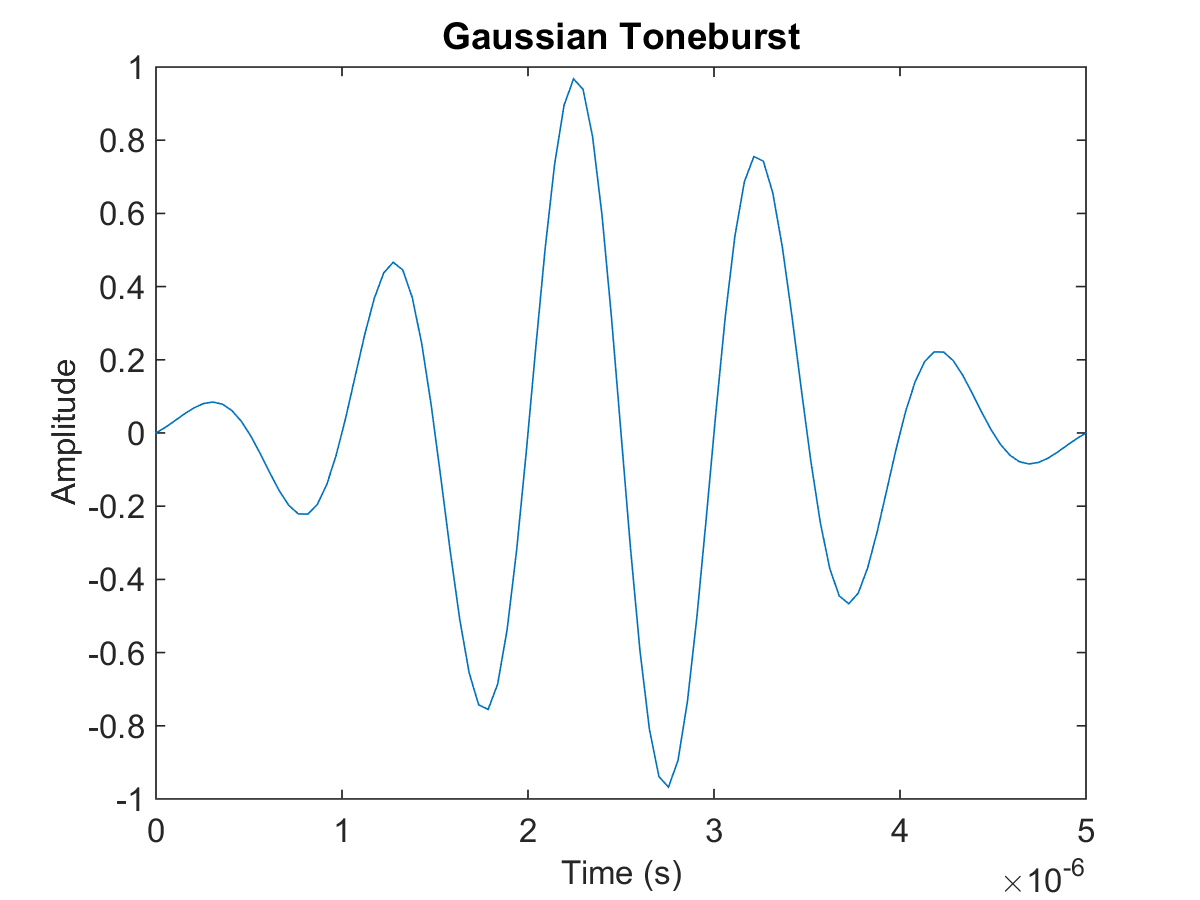
\includegraphics[width=100mm]{InitialToneburst.png}
		\caption{A Gaussian windowed toneburst of frequency 1MHz}
		\label{fig:cafi_toneburst}
\end{figure}

The moment when the tone-burst is applied to the system is labelled as time $t=0$. The combined A-scan trace without any correction for propagation delays is shown in Figure \ref{fig:cafi_isotropic1} below. The red trace represents $Rx1$ and the green trace represents $Rx2$.

\begin{figure}[htb]
\centering
		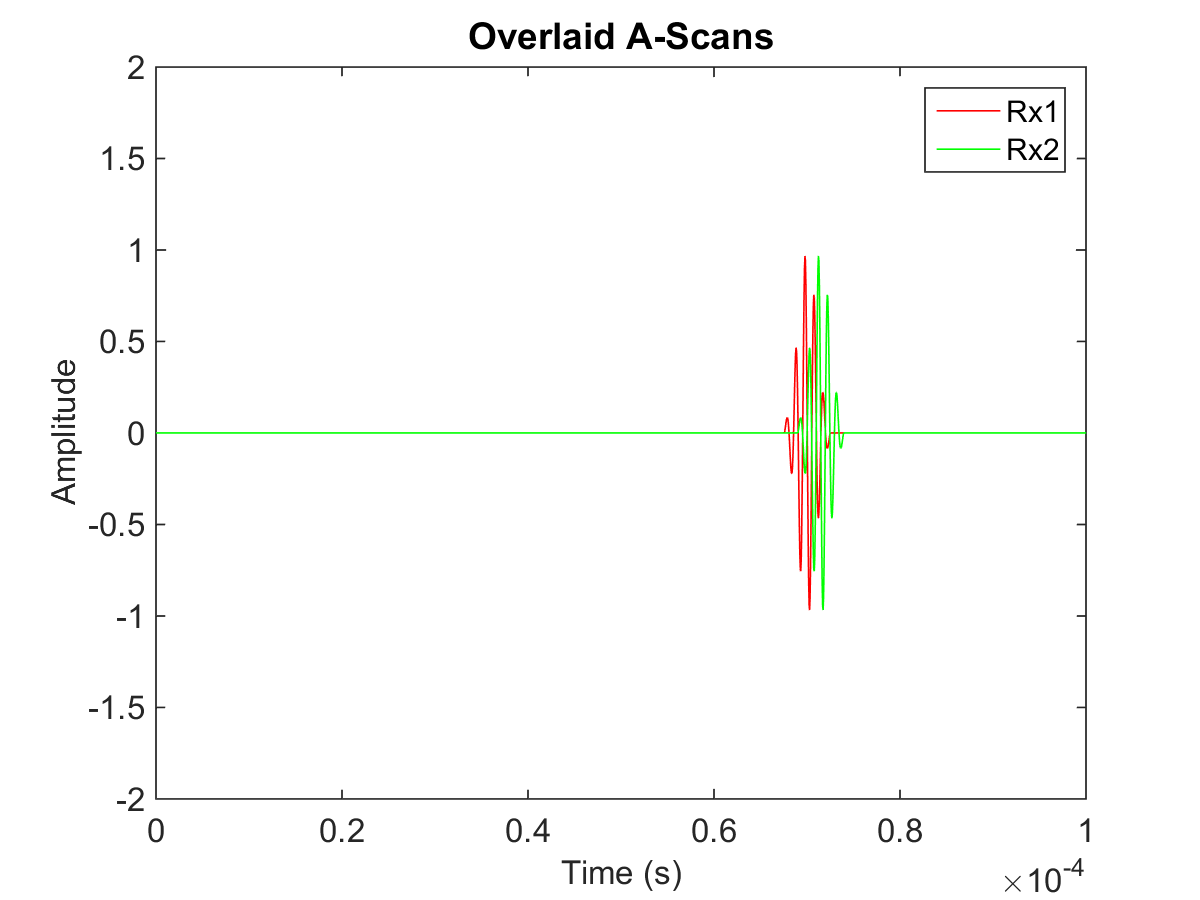
\includegraphics[width=100mm]{Isotropic_1.png}
		\caption{Two A-Scans overlaid without delay correction}
		\label{fig:cafi_isotropic1}
\end{figure}

\begin{figure}[htb]
\centering
		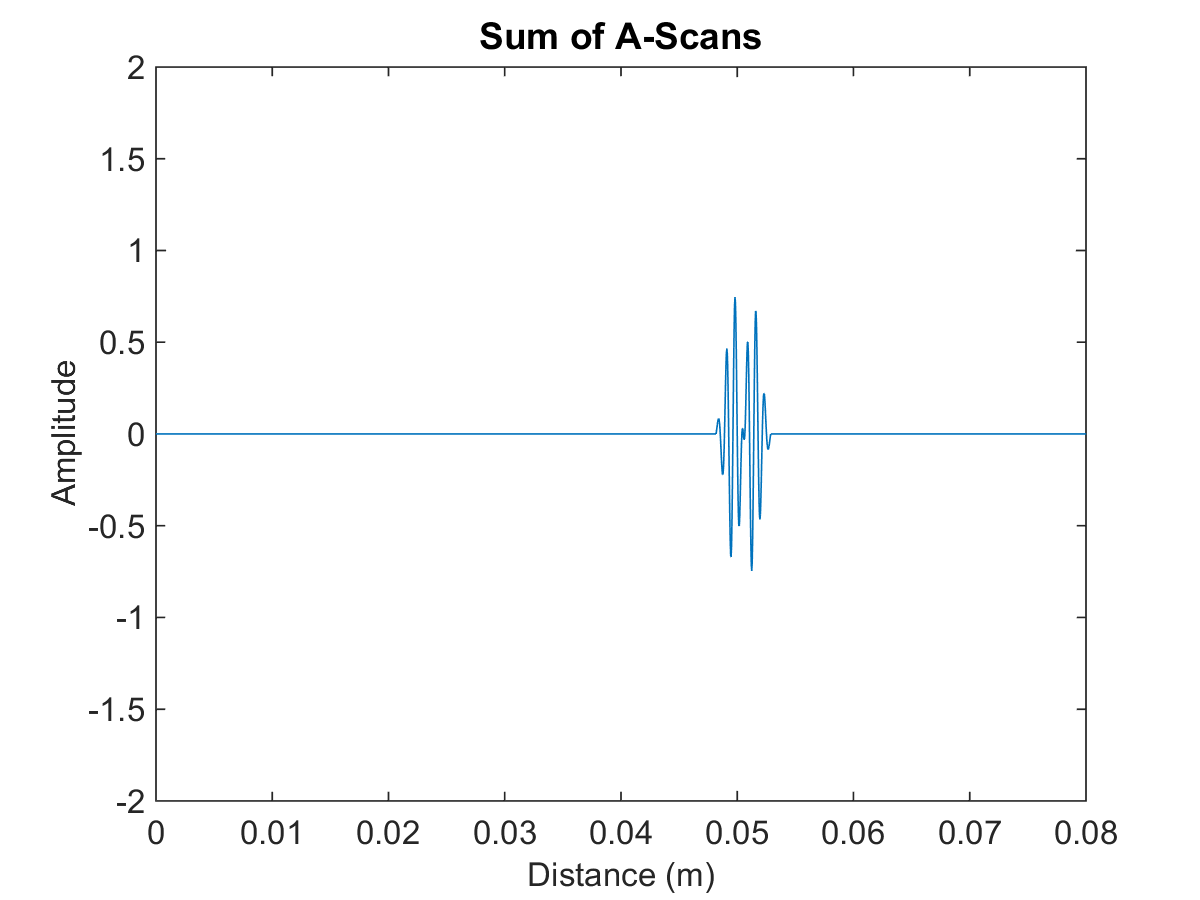
\includegraphics[width=100mm]{Isotropic_2.png}
		\caption{Two A-Scans combined without delay correction}
		\label{fig:cafi_isotropic2}
\end{figure}

The combined signal is shown in Figure \ref{fig:cafi_isotropic2}. Instead of overlaying the signals on top of each other, as in Figure \ref{fig:cafi_isotropic1}, they are now being summed together. It is apparent that the signals are interacting but constructive interference is not taking place due to the fact that the signals are not in phase. The maximum amplitude in the system is still less than 1 which is the maximum amplitude of our initial tone-burst. Using the knowledge of the location of the receiving sensors with respect to the transmitter, the round-trip delay can be calculated for each receiver. A lag (calculated by taking the difference between round-trip delays) can be applied to one of the signals, thus delaying it with respect to the other.

Equations \ref{eq:cafi_delays_general1} and \ref{eq:cafi_delays_general2} are used to calculate each of the delays where $V_{y,z}$ is the point reflector defined by its Cartesian coordinates. $t_{y,z}$ is the location the point of transmission and $r_{y,z}$ is the location of the receiver. These points can be related to the hypothetical experimental setup shown in Figure \ref{fig:cafi_experiment}. Equation set \ref{eq:cafi_delays_general1} calculates the distance between the point reflector and the other points of interest. $t_{path}$ and $r_{path}$ are the distances to and from the transmitting element to a pixel, $p$, and from the pixel to the receiving element, respectively.


\begin{subequations} \label{eq:cafi_delays_general1}
\begin{equation}  \label{eq:cafi_delays_general1_1}
t_{path} = \sqrt{(t_{y}-V_{y})^2 + (t_{z}-V_{z})^2}
\end{equation}

\begin{equation}  \label{eq:cafi_delays_general1_2}
r_{path} = \sqrt{(r_{y}-V_{y})^2 + (r_{z}-V_{z})^2}
 \end{equation}
\end{subequations}

Equation set \ref{eq:cafi_delays_general2} uses the times calculated in \ref{eq:cafi_delays_general1} to calculate the delays. Note that the delay is equal to the difference in time between the receive path and the transmit path, as everything is calculated relative to the point of transmission. This becomes essential when a number of receiving elements are employed as a static point of reference is required.

\begin{subequations} \label{eq:cafi_delays_general2}
\begin{equation}
delay = \frac{( r_{path} + t_{path} )  - ( t_{path} + t_{path} )}{v_L}
\end{equation}
\begin{equation}
delay = \frac{r_{path} - t_{path}}{v_L}
\end{equation}
\begin{equation}\label{eq:cafi_delays_general3}
delay = \frac{\sqrt{(r_{y}-V_{y})^2 + (r_{z}-V_{z})^2} - \sqrt{(t_{y}-V_{y})^2 + (t_{z}-V_{z})^2}}{v_L}
\end{equation}
\end{subequations}

For the example in Figure \ref{fig:cafi_experiment}, Equation \ref{eq:cafi_delays_general3} can be simplified further. It is known that the transmitter and receiver have the same $y$ co-ordinate and that the point reflector and the transmitter have the same $x$ co-ordinate. Taking this into account, the simplification shown in Equation \ref{eq:cafi_delays} can be derived. Note that this equation only holds true when the points of interest are orthogonal.

 \begin{equation} \label{eq:cafi_delays}
delay = \frac{\sqrt{V_{z}^2 + r_{y}^2} - V_{z} }{v_L}
 \end{equation}

The equation is essentially the propagation time from the transmitter to the point of interest minus the propagation time from the receiver to the point of interest. When applied to both receiving elements, the delayed signal can be seen as depicted in Figure \ref{fig:cafi_isotropic3}. Again, the red line is $Rx1$ and the green line is $Rx2$. It should be noted that due to the corrected delays, the lines are on top of each other, rendering the red line completely invisible. This is the expected and ideal case.

\begin{figure}[htb]
\centering
		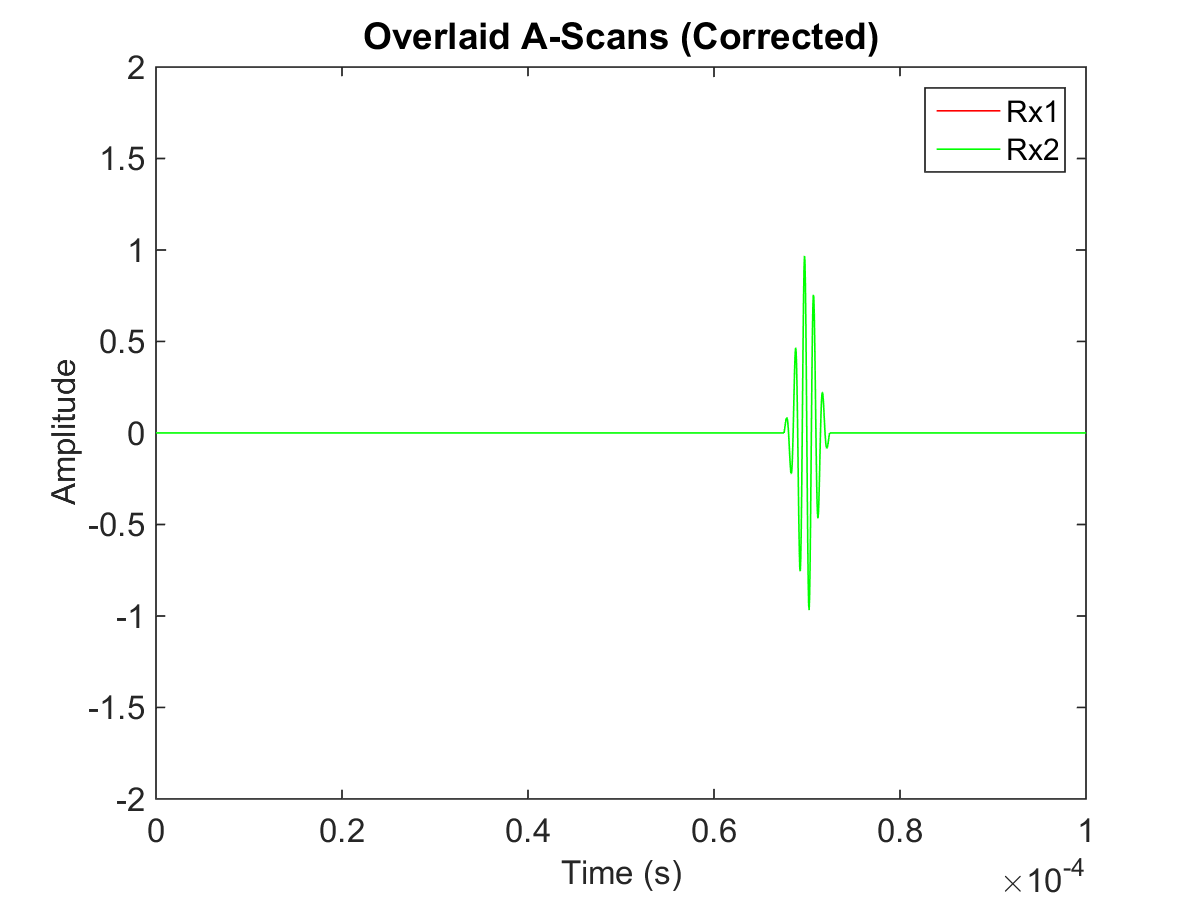
\includegraphics[width=100mm]{Isotropic_3.png}
		\caption{Two A-Scans overlaid with delay correction}
		\label{fig:cafi_isotropic3}
\end{figure}

The next image, in Figure \ref{fig:cafi_isotropic4}, shows the sum of both the individual A-scans. It can be observed the maximum amplitude is now 2, indicating that the signals are now summing constructively. The distance is also at the correct location, at 0.05 meters which is the location of the simulated point reflector.

\begin{figure}[htb]
\centering
		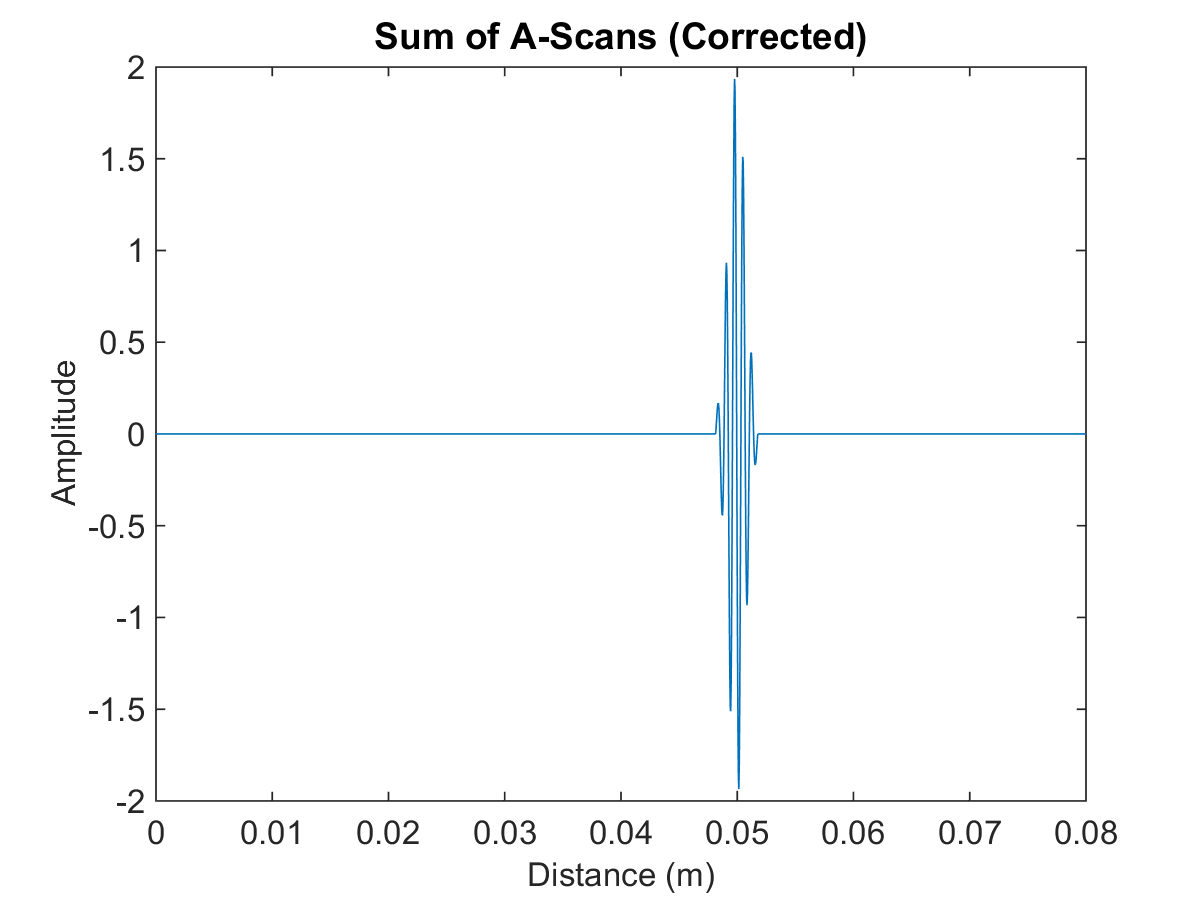
\includegraphics[width=100mm]{Isotropic_4.png}
		\caption{Two A-Scans combined delay correction}
		\label{fig:cafi_isotropic4}
\end{figure}
\clearpage

\subsubsection{Nearest Neighbour Cross-Correlation in Anisotropic Materials}

Delay-and-sum processing has been considered for a simple system. Let us now add a layer of complexity to our system. Difficult materials, besides being highly scattering and attenuating, are generally anisotropic. That is, having properties that are directionally dependent. Often, a wave will propagate in one direction at a differing speed from other directions. This hinders the ability to effectively delay and sum contributions from different receivers. An example of this is now presented.

\begin{figure}[htb]
\centering
		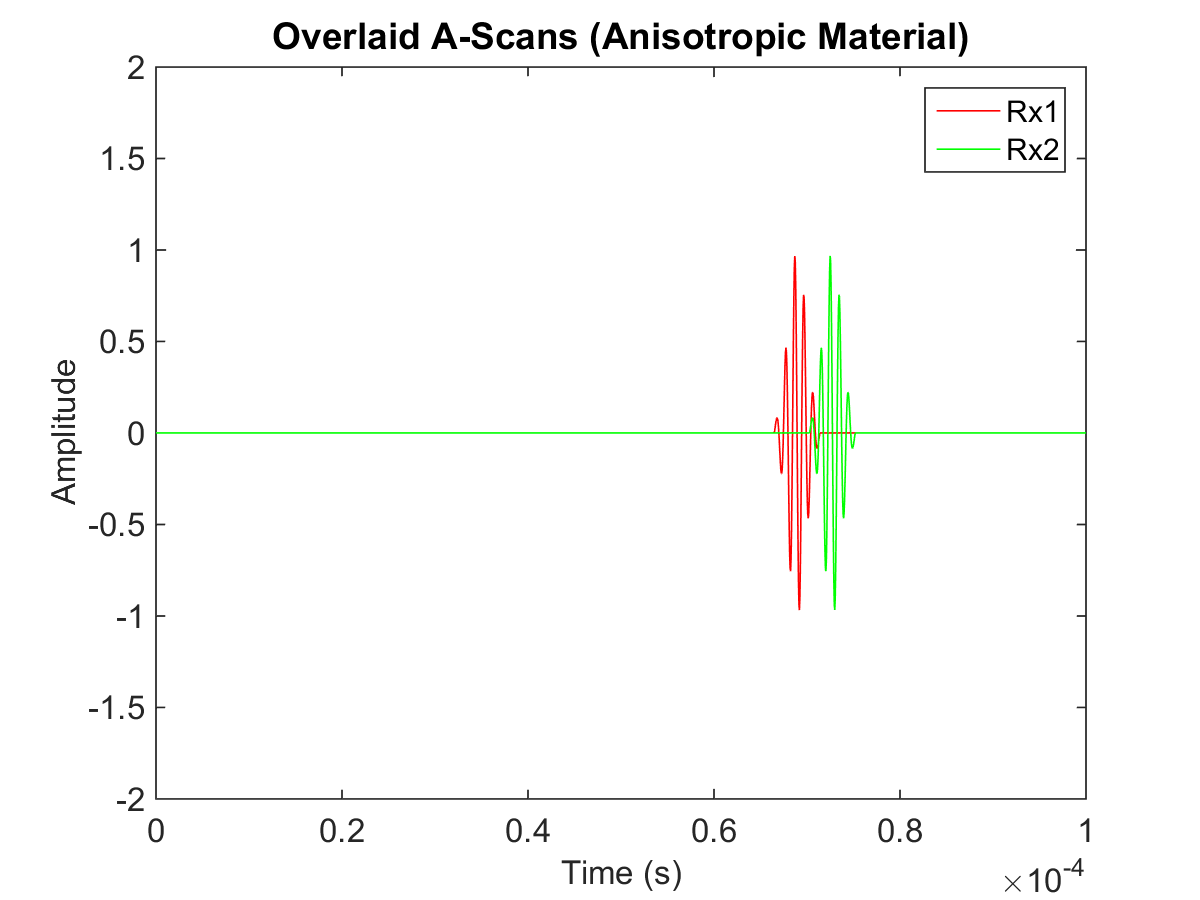
\includegraphics[width=100mm]{Anisotropic_1.png}
		\caption{Two A-Scans overlaid without delay correction (anisotropic model)}
		\label{fig:cafi_anisotropic1}
\end{figure}

\begin{figure}[htb]
\centering
		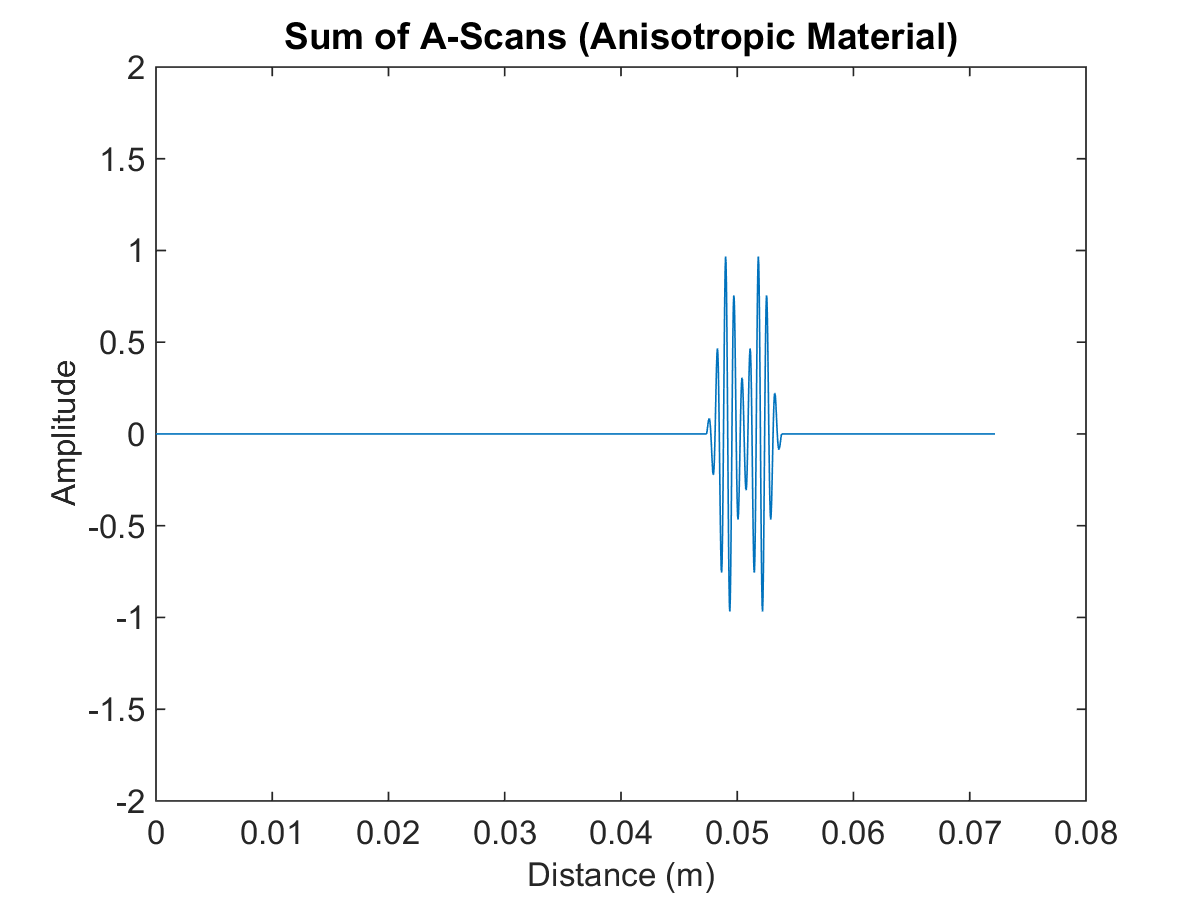
\includegraphics[width=100mm]{Anisotropic_2.png}
		\caption{Two A-Scans combined without delay correction (anisotropic model)}
		\label{fig:cafi_anisotropic2}
\end{figure}


The same hypothetical arrangement is used as shown in Figure \ref{fig:cafi_experiment}, only now the wave velocity from $p$ to $Rx1$ is 1530m/s and the wave velocity from $p$ to $Rx2$ is 1430m/s. Figures \ref{fig:cafi_anisotropic1} and \ref{fig:cafi_anisotropic2} show that without accounting for propagation time everything looks much the same as in the more simple scenario. Figure \ref{fig:cafi_anisotropic3} is different compared to Figure \ref{fig:cafi_isotropic3}, as both A-scans are visible now. The waves are no longer co-incident with each other and when Figure \ref{fig:cafi_anisotropic4} is observed, the waves are no longer summing constructively and the maximum amplitude is reduced to 1. It can be observed that a deviation of just 3\% from the assumed propagation velocity (1480m/s) is enough to stop delay and sum imaging from working correctly. 

\begin{figure}[htb]
\centering
		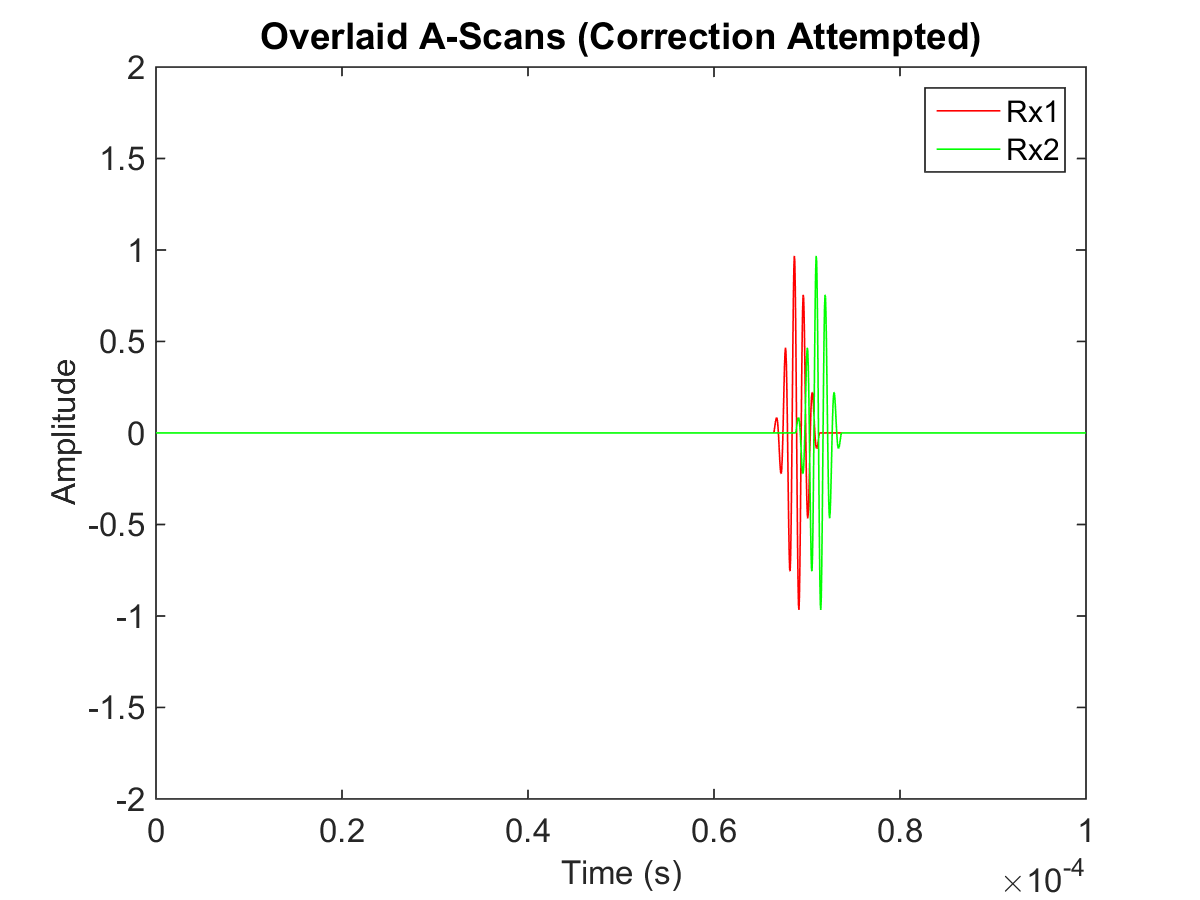
\includegraphics[width=100mm]{Anisotropic_3.png}
		\caption{Two A-Scans overlaid with attempted delay correction (anisotropic model)}
		\label{fig:cafi_anisotropic3}
\end{figure}

\begin{figure}[htb]
\centering
		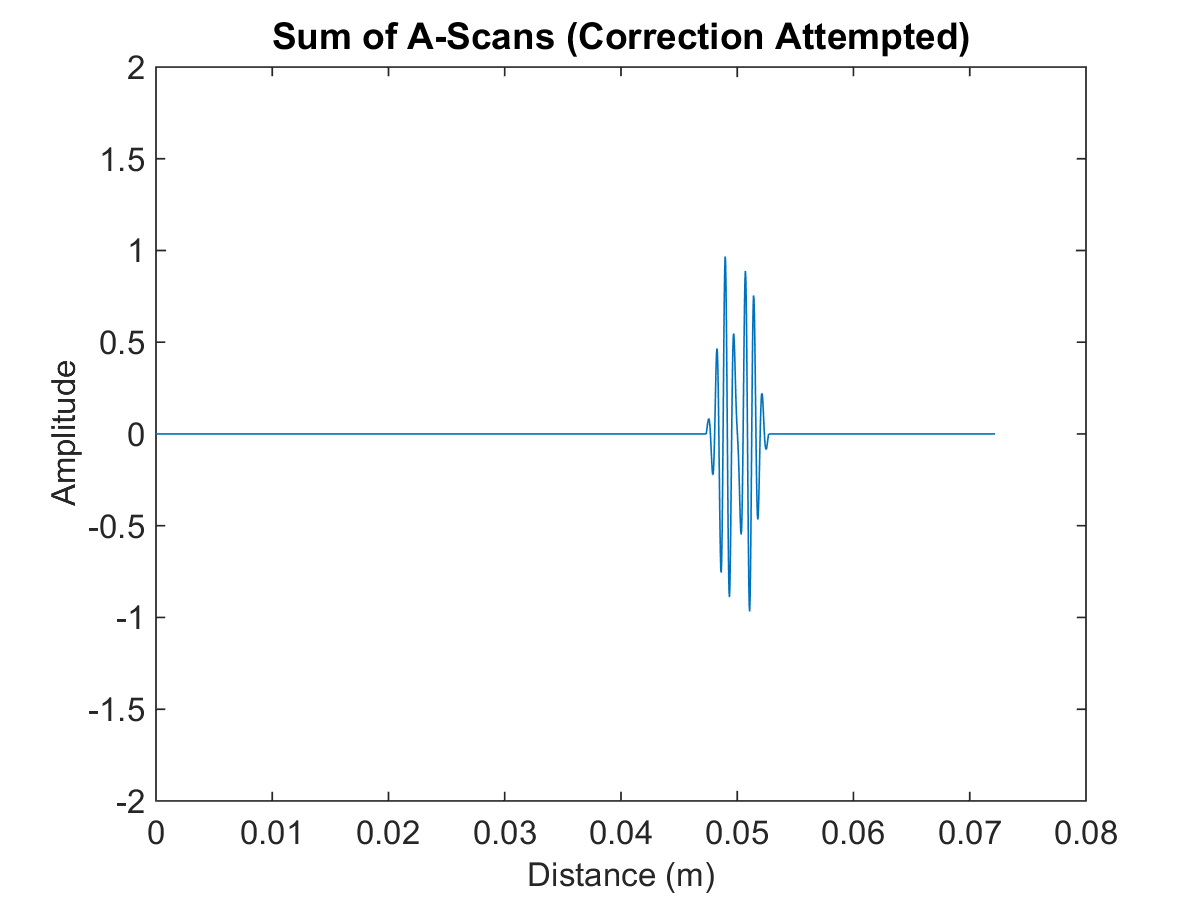
\includegraphics[width=100mm]{Anisotropic_4.png}
		\caption{Two A-Scans combined with attempted delay correction (anisotropic model)}
		\label{fig:cafi_anisotropic4}
\end{figure}

\begin{figure}[htb]
\centering
		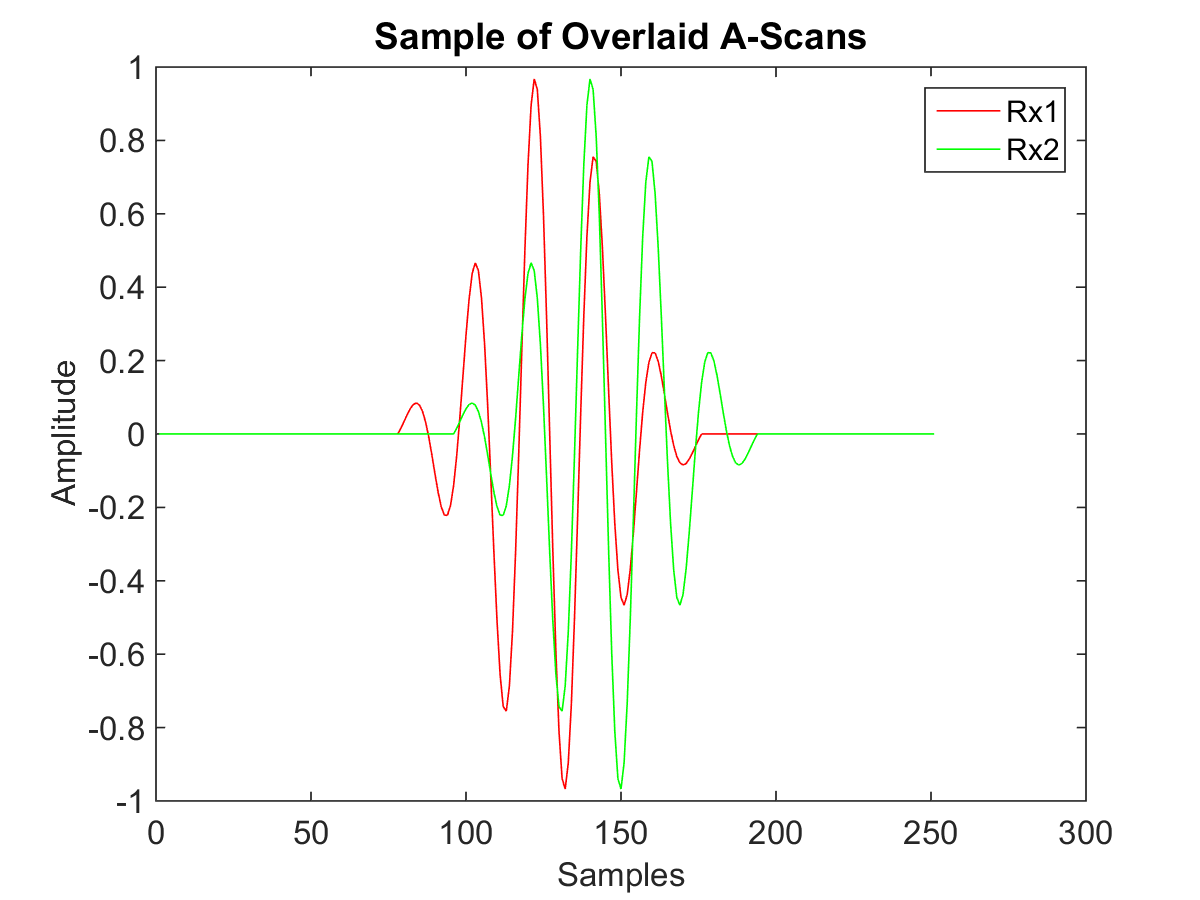
\includegraphics[width=100mm]{Anisotropic_5.png}
		\caption{A section of the overlaid A-Scans before cross-correlation}
		\label{fig:cafi_anisotropic5}
\end{figure}

Figure \ref{fig:cafi_anisotropic5} shows a snapshot of the two signals. The estimated delays of the signal are known and with this knowledge, the area where the reflections occur can be extracted. Within this plot there is no knowledge of where the reflections are, but the anisotropy is assumed to be mild enough that the desired reflection will be in the area selected for cross-correlation.

The signals can be cross-correlated to find out the delay correction that would result in the highest cross-correlation coefficient between the two signals. This is found using Equation \ref{eq:cafi_xcorr} over a range of delays. Figure \ref{fig:cafi_anisotropic10} shows a plot of lags against cross-correlation coefficient. The maximum value of this plot is taken to be the optimum refined delay for the pair of A-Scans, which for this case was found to be 18.

\begin{figure}[htb]
\centering
		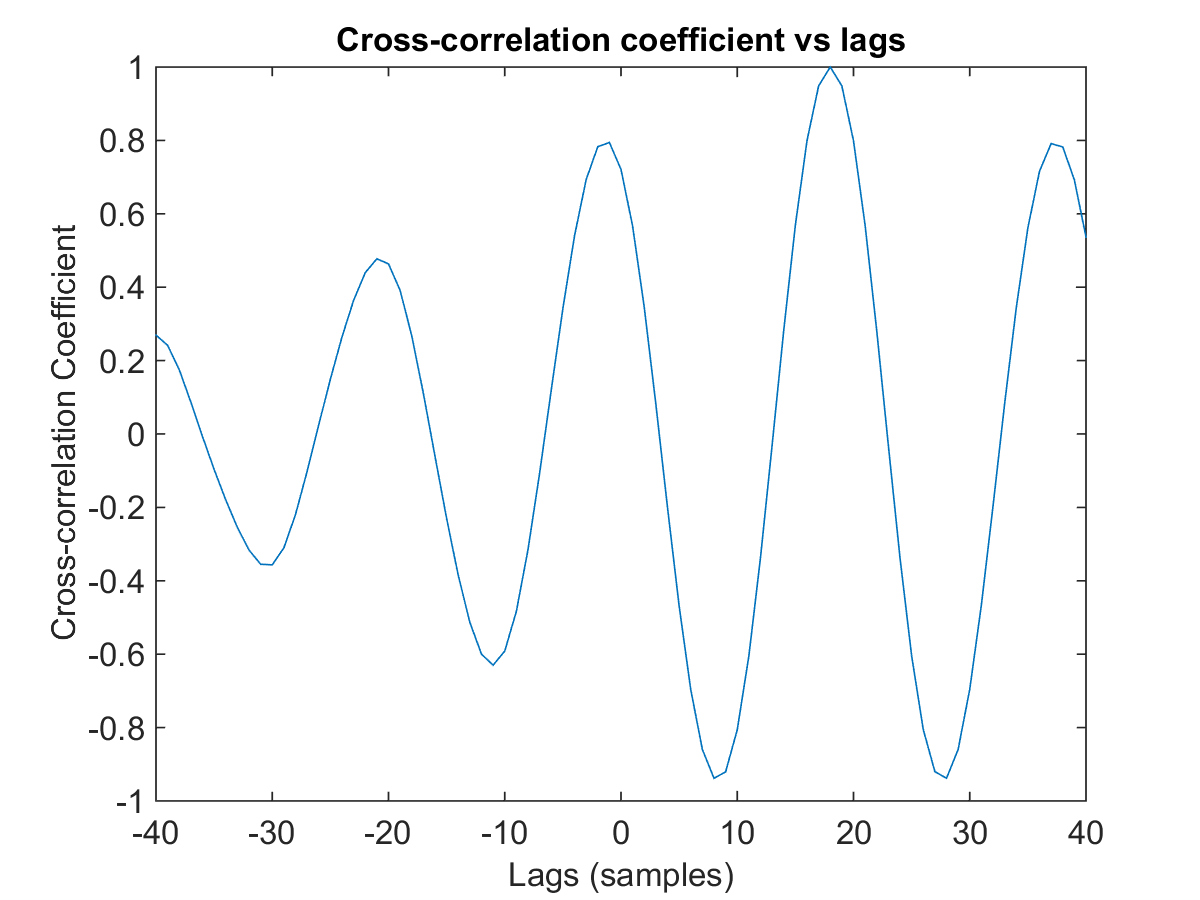
\includegraphics[width=100mm]{Anisotropic_10.png}
		\caption{A plot of tested delays vs cross-correlation coefficient for the A-scans in Figure \ref{fig:cafi_anisotropic5}}
		\label{fig:cafi_anisotropic10}
\end{figure}

\begin{figure}[htb]
\centering
		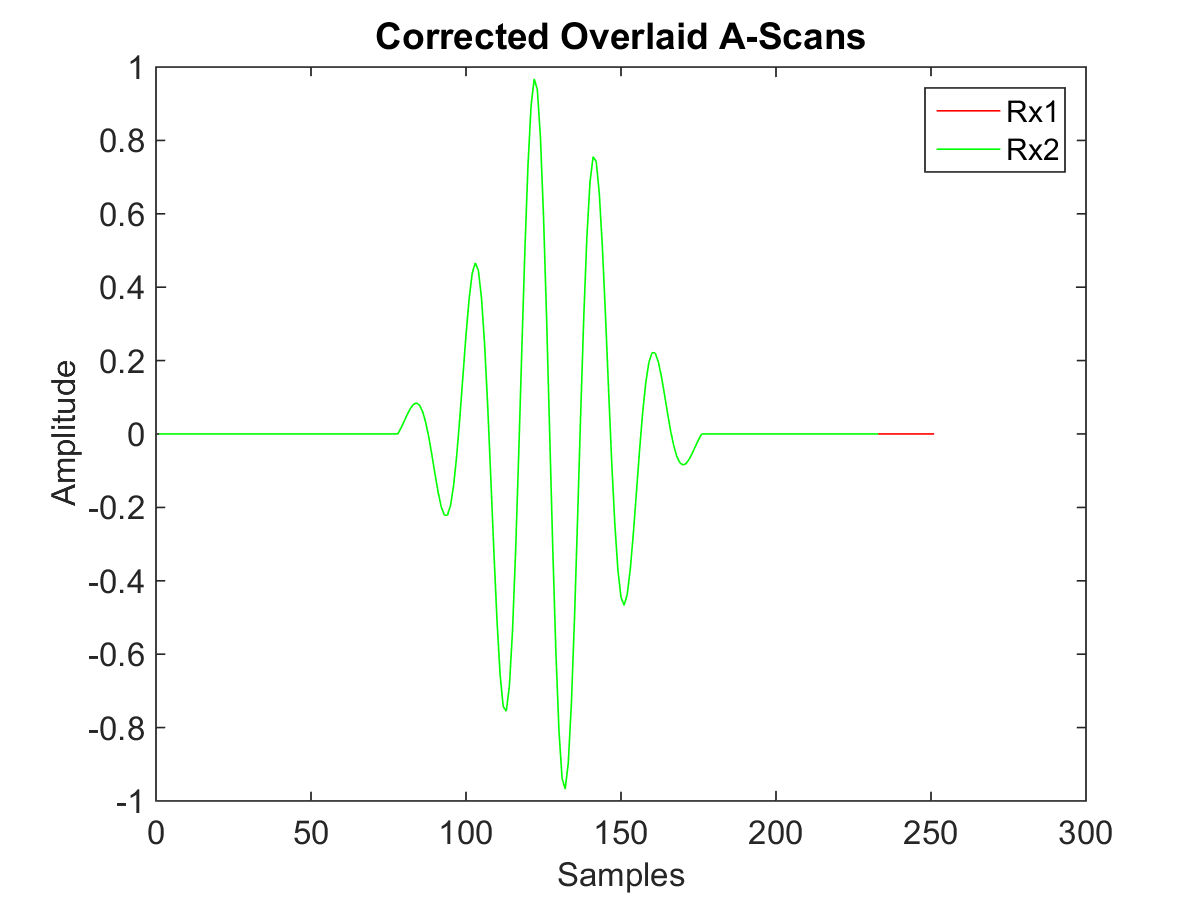
\includegraphics[width=100mm]{Anisotropic_6.png}
		\caption{A section of the overlaid A-Scans after cross-correlation and delay correction}
		\label{fig:cafi_anisotropic6}
\end{figure}


Figure \ref{fig:cafi_anisotropic6} shows the overlaid A-scans when the delay of 18 samples was applied to the second A-scan. The signals recombine and overlap as expected. Applied to the full A-scan, the final expected result can be seen in Figure \ref{fig:cafi_anisotropic7} and the combined result in Figure \ref{fig:cafi_anisotropic8}. Note that the location of the reflector has appeared to have moved slightly, from 0.5m to 0.49m. This is due to the fact that perfect delays cannot be applied due to the unknown precise velocities in the model. This error is low (2\%) and is a consequence of using NNCC to inform the CAFI algorithm.

\begin{figure}[htb]
\centering
		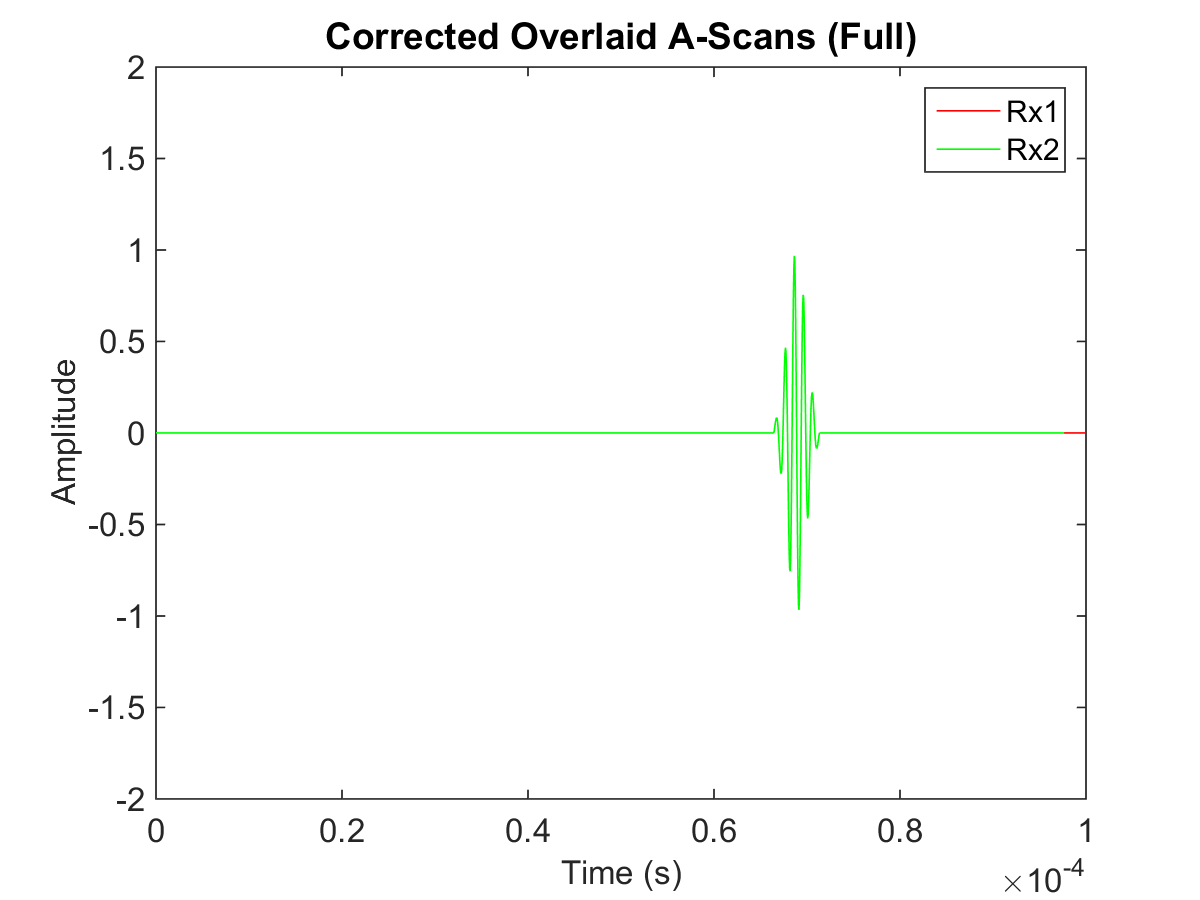
\includegraphics[width=100mm]{Anisotropic_7.png}
		\caption{Two A-Scans overlaid with CAFI correction}
		\label{fig:cafi_anisotropic7}
\end{figure}

\begin{figure}[htb]
\centering
		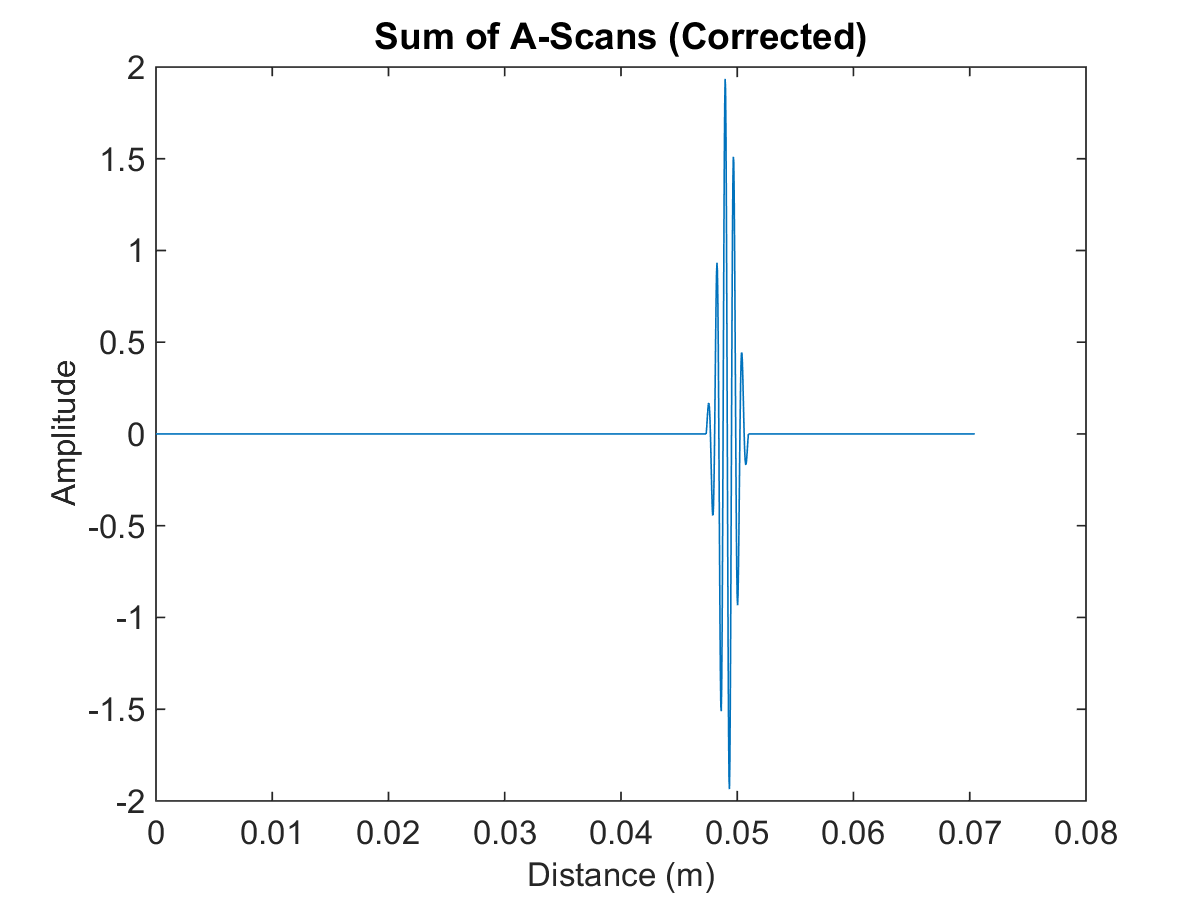
\includegraphics[width=100mm]{Anisotropic_8.png}
		\caption{Two A-Scans combined with CAFI correction}
		\label{fig:cafi_anisotropic8}
\end{figure}
\clearpage
\subsection{Nearest Neighbour Cross-Correlation in the Presence of Noise}

For NNCC-based imaging algorithms to be applicable in this work, they need to be robust in the presence of noise. In the next simulation, random noise is added to each A-scan. The peak amplitude of the toneburst is 1 and the peak amplitude of the noise is 1.5. This yields a signal to noise ratio of -3dB.

The combined delay-and-sum signal before NNCC correction is attempted is shown in Figure \ref{fig:cafi_noise4}.

\begin{figure}[htb]
\centering
		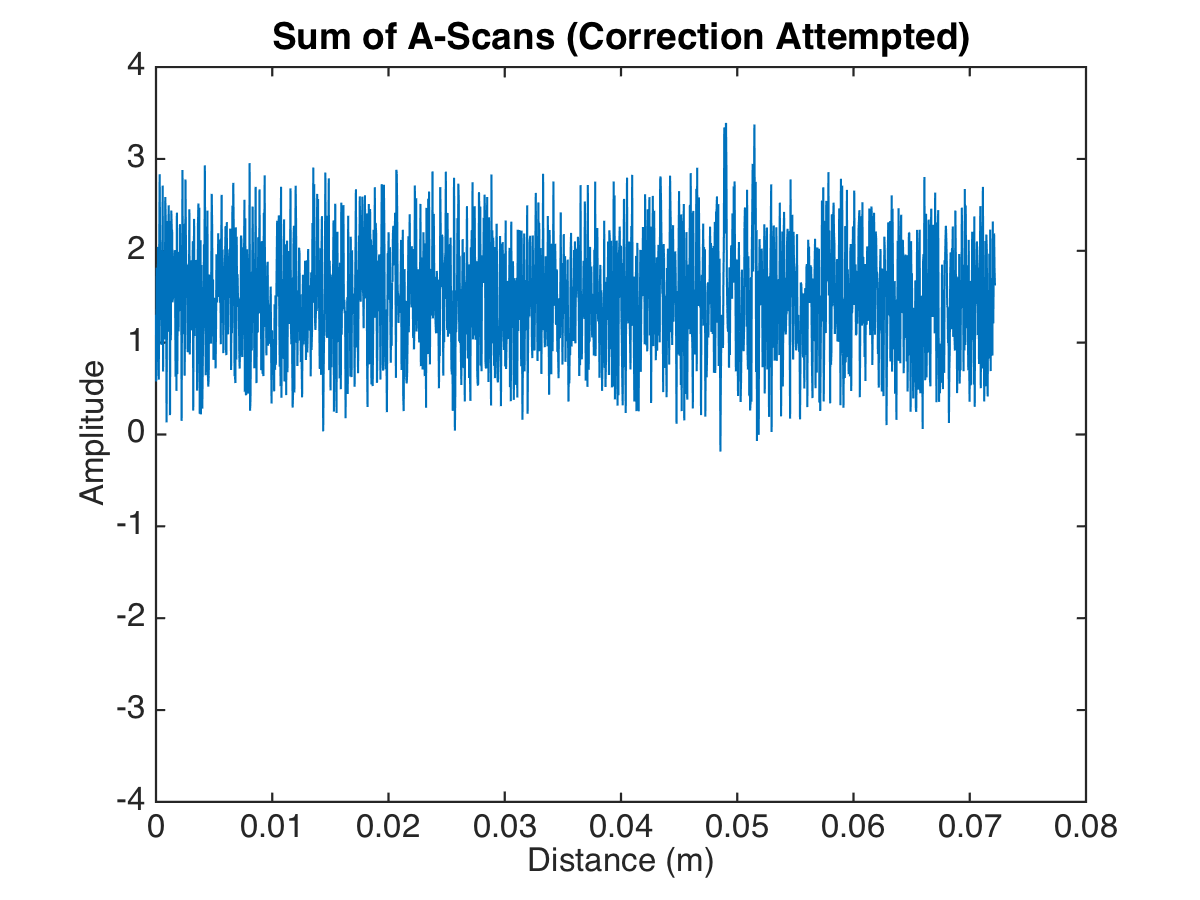
\includegraphics[width=100mm]{Noise_4.png}
		\caption{Two A-Scans combined with added noise}
		\label{fig:cafi_noise4}
\end{figure}

In Figure \ref{fig:cafi_noise4} there is a peak at 0.05m, but it is not clear if that is the result of noise or an actual feature. In this case, it is possible for the noise in each signal to undergo constructive interference and appear as a legitimate reflector in the combined A-scan. In the next set of images, Figures \ref{fig:cafi_noise5} to \ref{fig:cafi_noise8}, the CAFI technique is applied to the noisy signal to attempt to refocus the delay-and-sum A-Scan on the reflector.

\begin{figure}[htb]
\centering
		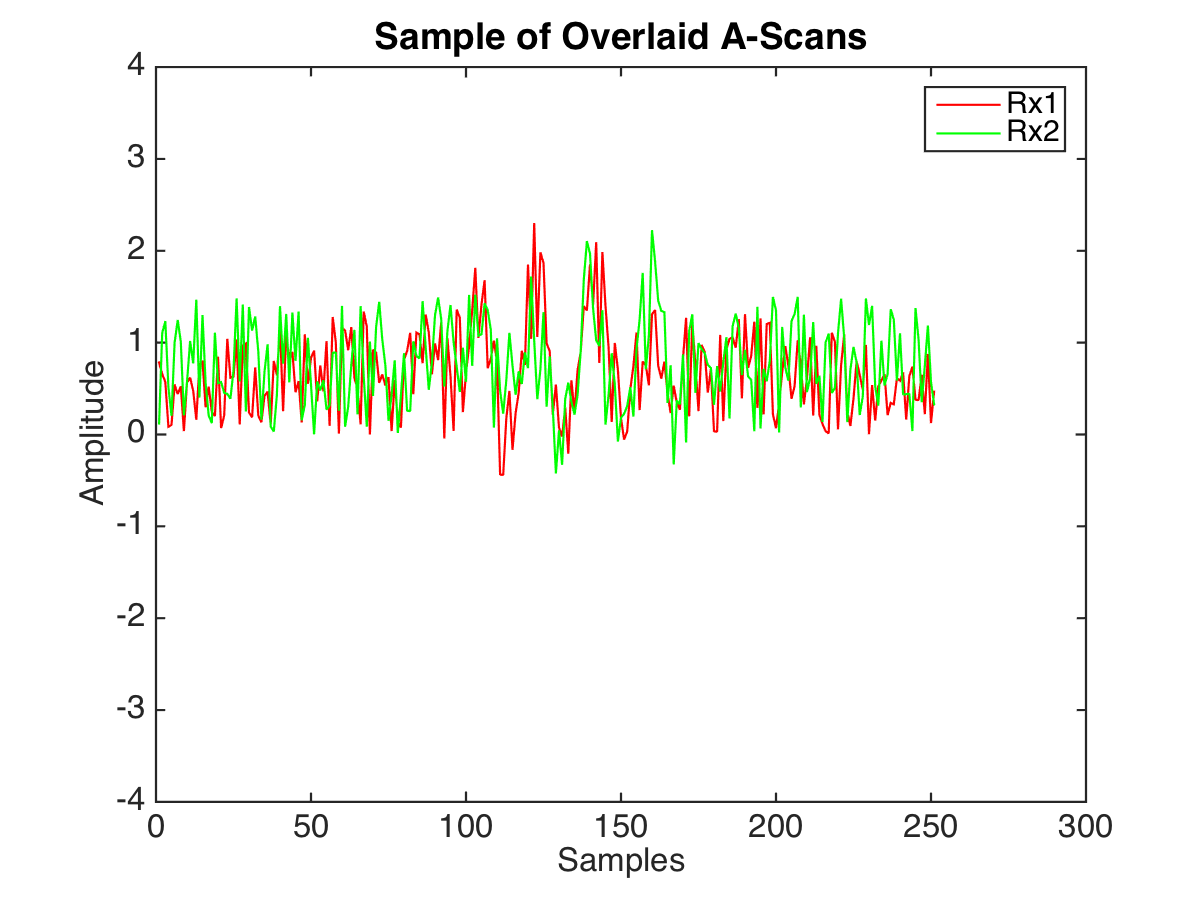
\includegraphics[width=100mm]{Noise_5.png}
		\caption{A subset of two A-Scans overlaid with added noise}
		\label{fig:cafi_noise5}
\end{figure}
\begin{figure}[htb]
\centering
		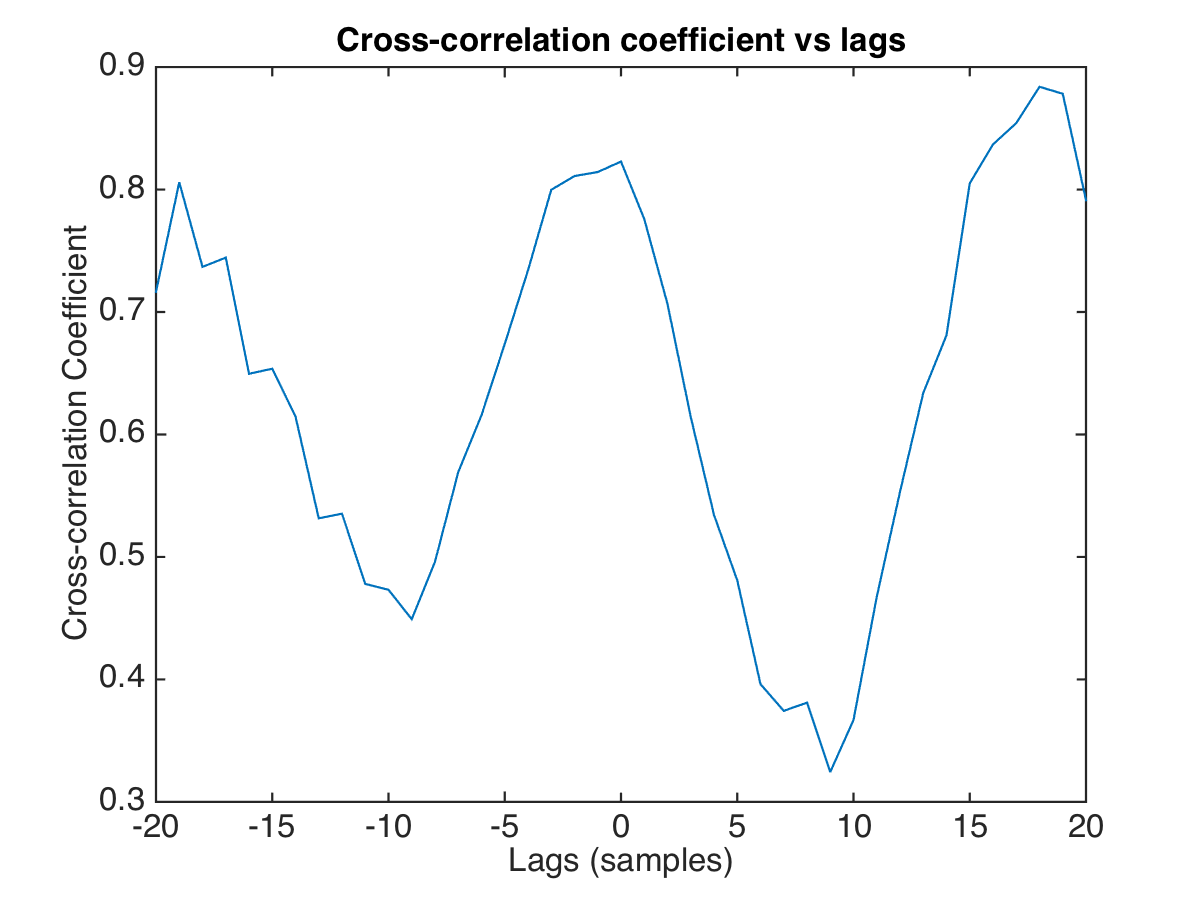
\includegraphics[width=100mm]{Noise_10.png}
		\caption{A plot of tested delays vs cross-correlation coefficient for the A-scans in Figure \ref{fig:cafi_noise5}}
		\label{fig:cafi_noise10}
\end{figure}
\begin{figure}[htb]
\centering
		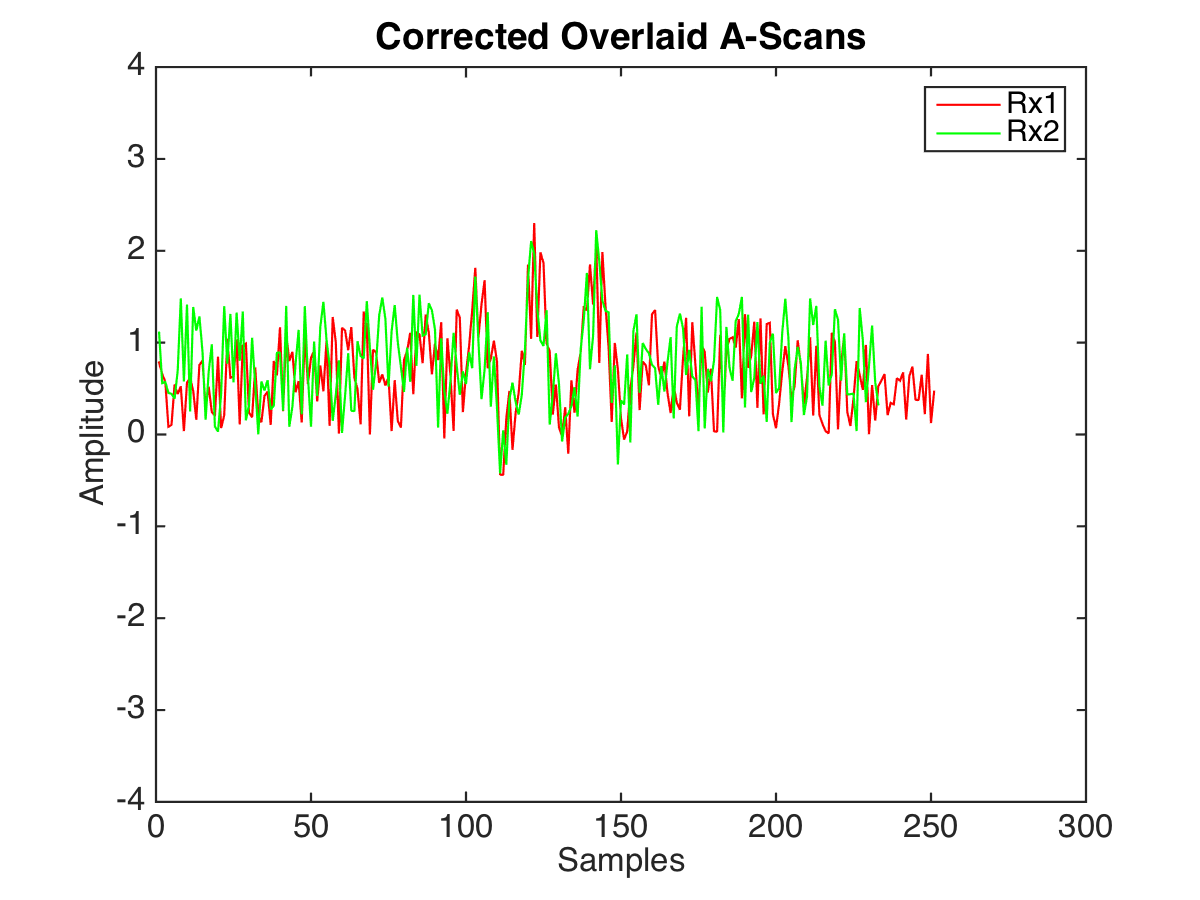
\includegraphics[width=100mm]{Noise_6.png}
		\caption{A subset of two A-Scans overlaid with added noise and corrected using CAFI}
		\label{fig:cafi_noise6}
\end{figure}
\begin{figure}[htb]
\centering
		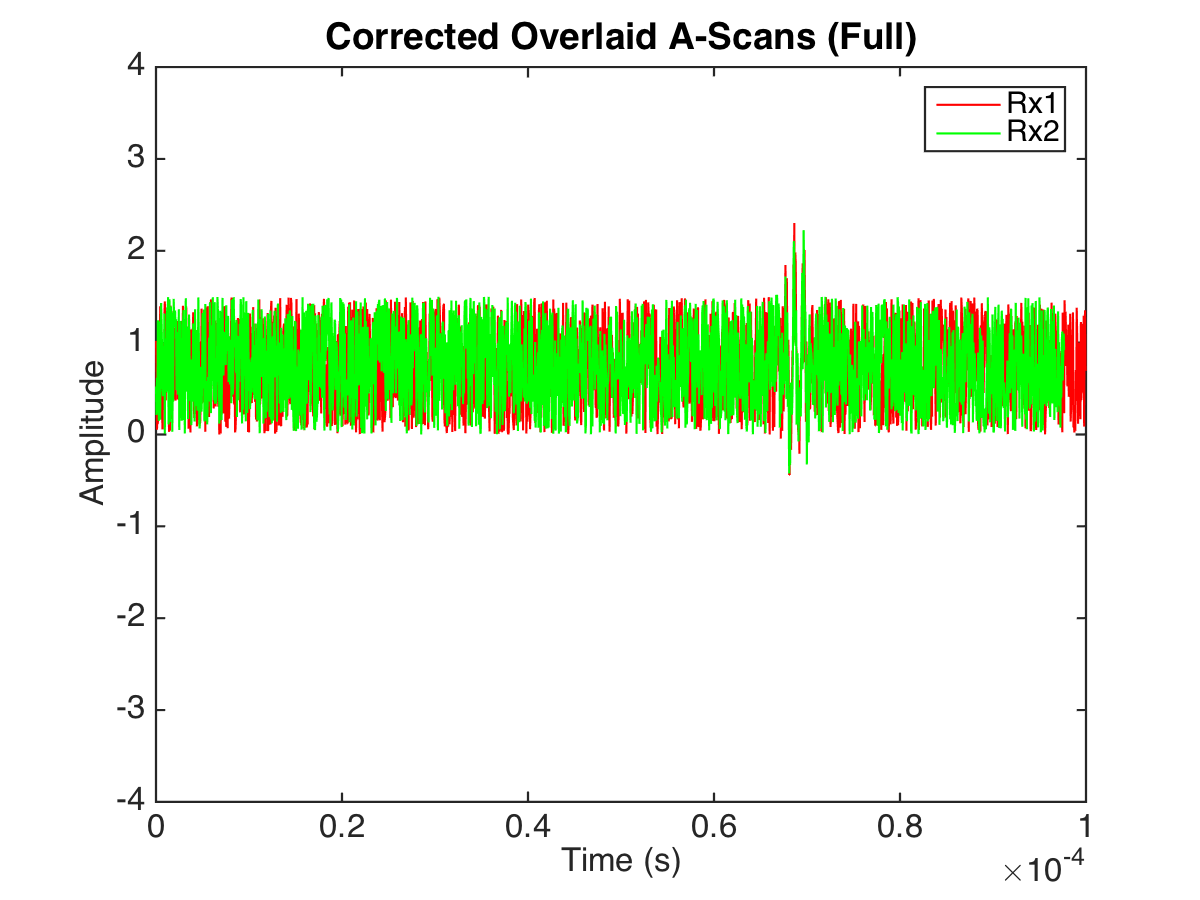
\includegraphics[width=100mm]{Noise_7.png}
		\caption{Two A-Scans overlaid with added noise and corrected using CAFI}
		\label{fig:cafi_noise7}
\end{figure}
\begin{figure}[htb]
\centering
		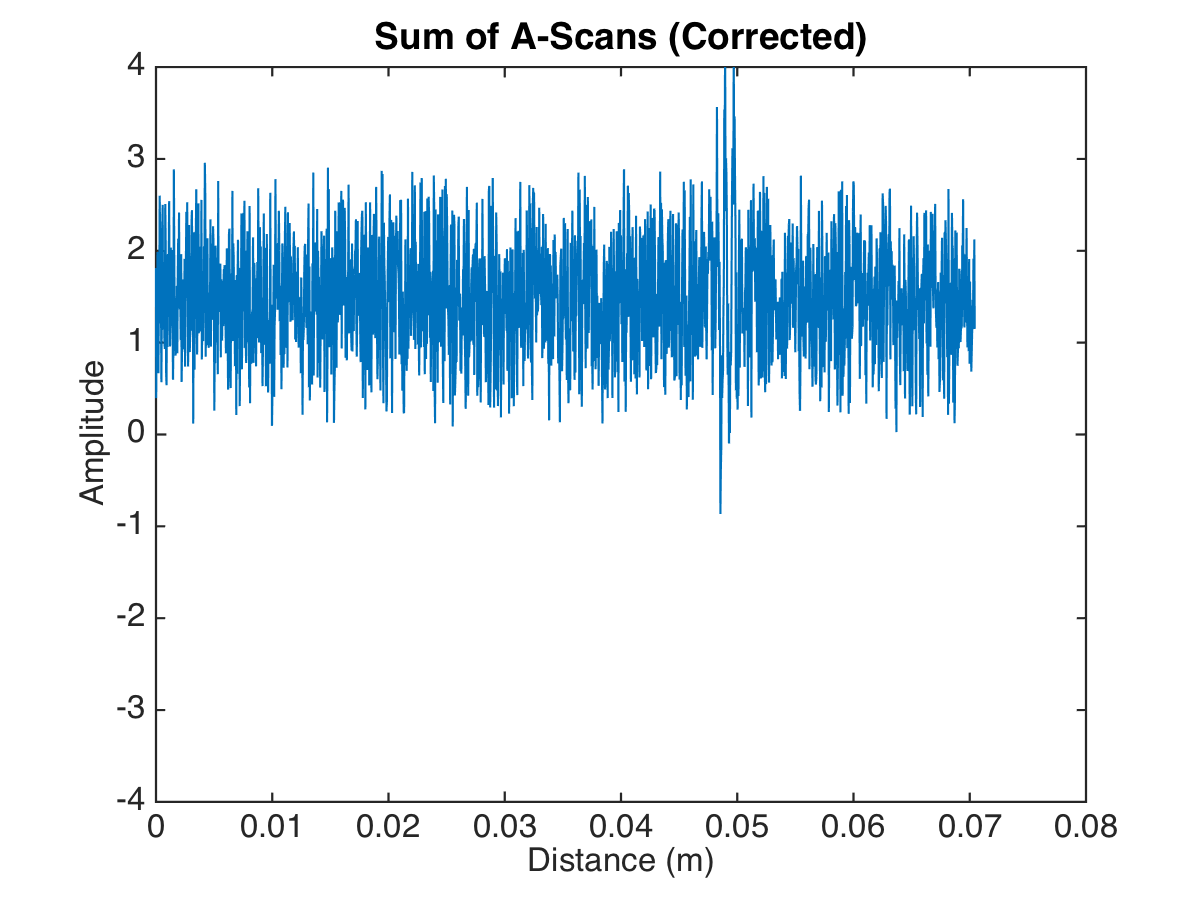
\includegraphics[width=100mm]{Noise_8.png}
		\caption{Two A-Scans combined with added noise and corrected using CAFI}
		\label{fig:cafi_noise8}
\end{figure}

Figure \ref{fig:cafi_noise10} shows the cross-correlation coefficient against lags for the noisy signal. When compared with a clean signal such as the one in the previous example, shown in Figure \ref{fig:cafi_anisotropic10}, the peak indicating the correct number of lags can be seen to be less prominent. The ideal delay can be observed from the graph to be 19 samples. This differs from the previous example by only one sample, or 50ns.

Comparing the before and after, Figures \ref{fig:cafi_noise4} and \ref{fig:cafi_noise8} respectively, there is a marked improvement in effective SNR. The SNR in the after image (peak signal to peak noise) is 3.0, while in the before image the SNR is 1.4. This may seem like a small difference but it shows an increase of SNR of 110\%, over double the original SNR. Qualitatively, there is clearly a reflector shown at 0.05m. This is an improvement over the `before' image.
\clearpage
\subsection{Phase Enhanced Correlation for Adaptively Focused Imaging}

The focus correction can be altered by using a different way to measure the signal in the cross-correlation. Using the instantaneous phase of a signal for comparison means that the cross-correlation algorithm no longer depends on signal amplitude. This makes CAFI more resilient to high amplitude noise that is typically found when inspecting coarse grain materials\cite{camacho_phase_2011}. Applying the Hilbert transform to an RF signal yields the analytical signal with both real and imaginary components, as seen in \ref{fig:cafi_phases}. The instantaneous phase is calculated for each sample by calculating the phase angle,$\phi_{0}$, between the real and imaginary components of said sample.

\begin{figure}[hp]
\centering
		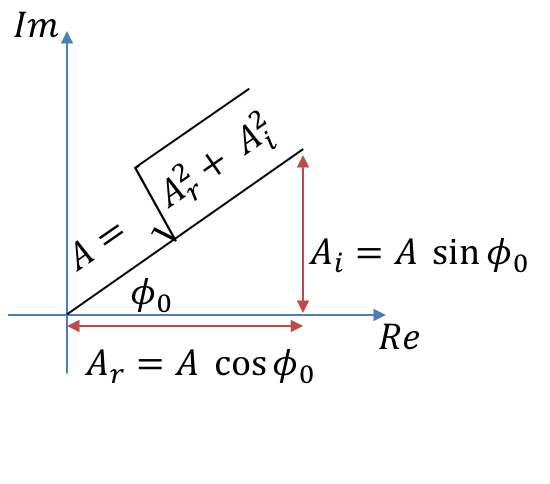
\includegraphics[width=100mm]{Phases2.png}
		\caption{Finding the phase of an analytical signal using the real and imaginary components}
		\label{fig:cafi_phases}
\end{figure}

The CAFI process can then be repeated using the instantaneous phases as an input to the cross-correlation algorithm, in place of a signal's amplitude. Once the ideal delays have been calculated, the delay and sum imaging can take place as before using the original A-Scans. Again, this concept will be demonstrated on the noisy anisotropic model.

\begin{figure}[hp]
\centering
		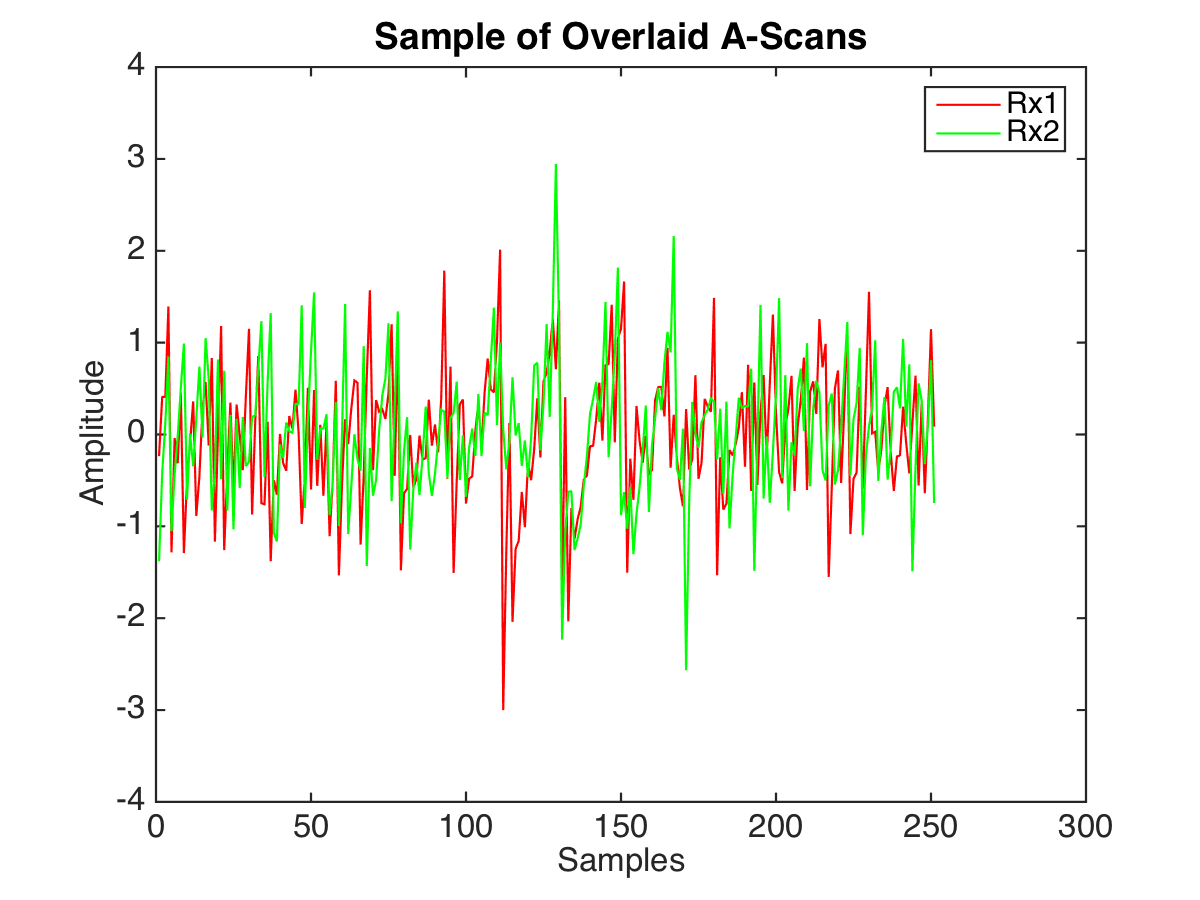
\includegraphics[width=100mm]{Noise_5_Phase.png}
		\caption{Overlaid subset of instantaneous phases}
		\label{fig:cafi_phase5}
\end{figure}

\begin{figure}[hp]
\centering
		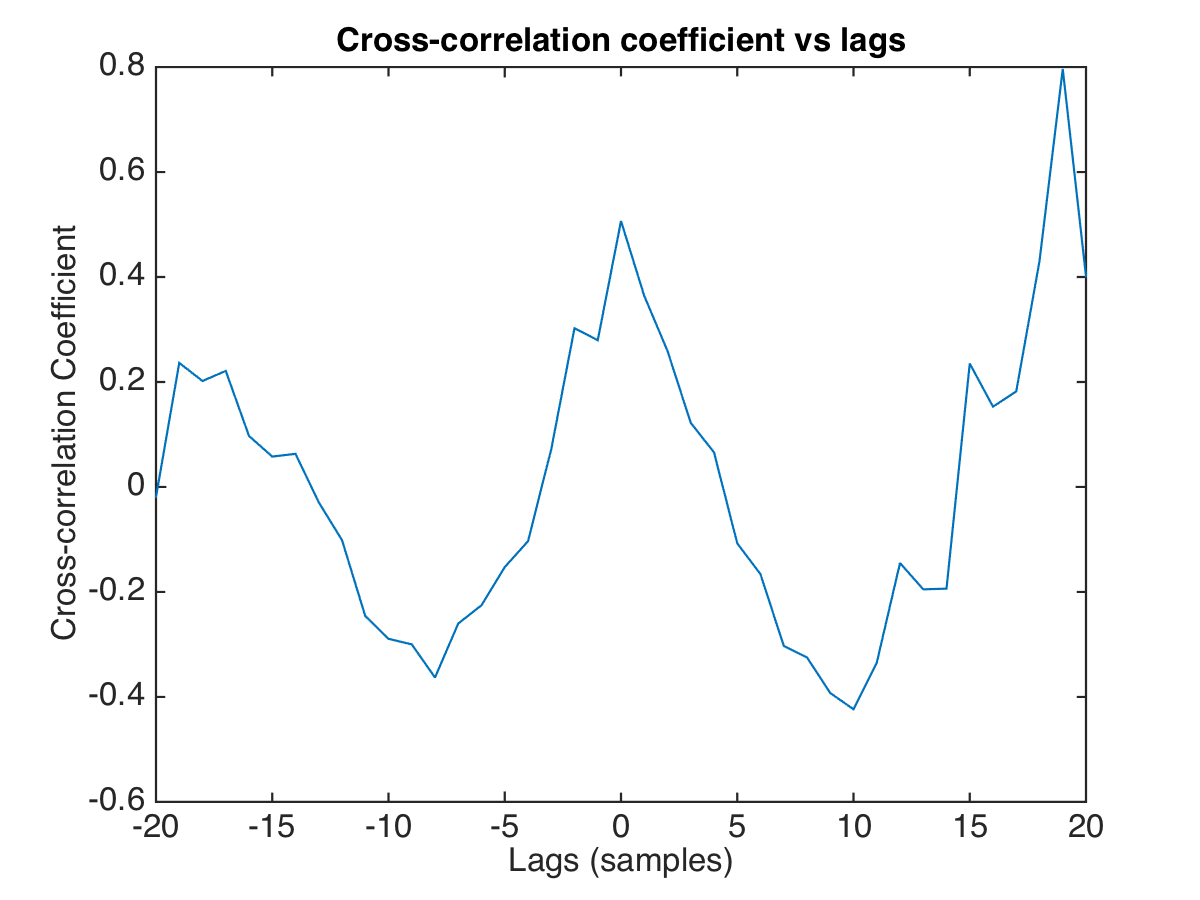
\includegraphics[width=100mm]{Noise_10_Phase.png}
		\caption{A plot of tested delays vs cross-correlation coefficient for the A-scans in Figure \ref{fig:cafi_phase5}}
		\label{fig:cafi_phase10}
\end{figure}

Figure \ref{fig:cafi_phase5} shows a sample of the A-scans, overlaid on each other, after the instantaneous phase angle has been calculated. These signals are then input to the cross-correlation function, the results of which are shown in Figure \ref{fig:cafi_phase10}. The graph shows that the ideal delay is 18 samples, which is the expected value, given knowledge of the parameters of the hypothetical imaging scenario. This is an improvement over the standard `amplitude-only' CAFI using result which yielded an `ideal' delay of 19 samples. Furthermore, the graph is much steeper than the one generated from the amplitude-only CAFI. This is a property which can help to reduce false positives. Delays which are not optimal now have a much lower cross-correlation coefficient in the phase-based CAFI implementation. 

This correct delay is then applied and can be seen in Figures \ref{fig:cafi_phase6} to \ref{fig:cafi_phase8}.

\begin{figure}[hp]
\centering
		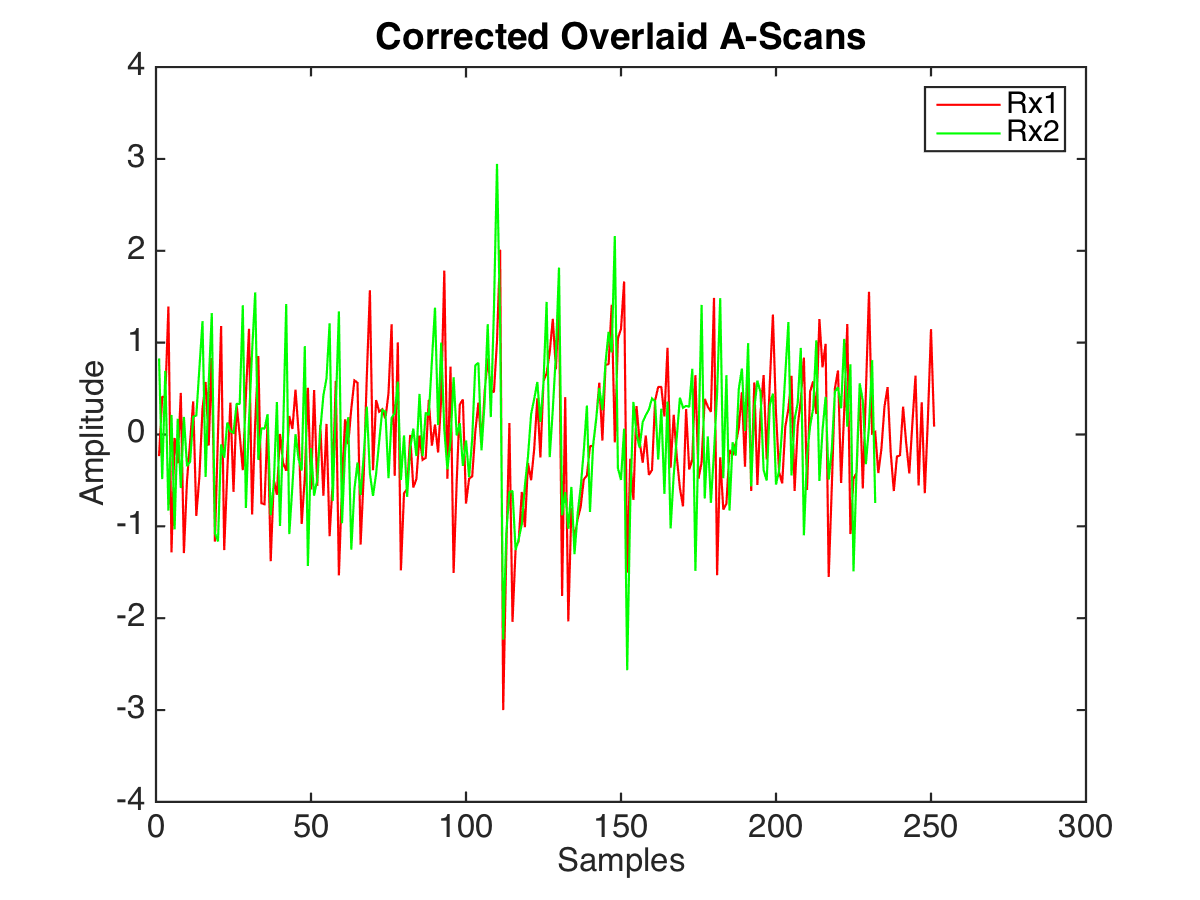
\includegraphics[width=100mm]{Noise_6_Phase.png}
		\caption{A subset of two A-scans' instantaneous phases overlaid with added noise and corrected using CAFI}
		\label{fig:cafi_phase6}
\end{figure}
\begin{figure}[hp]
\centering
		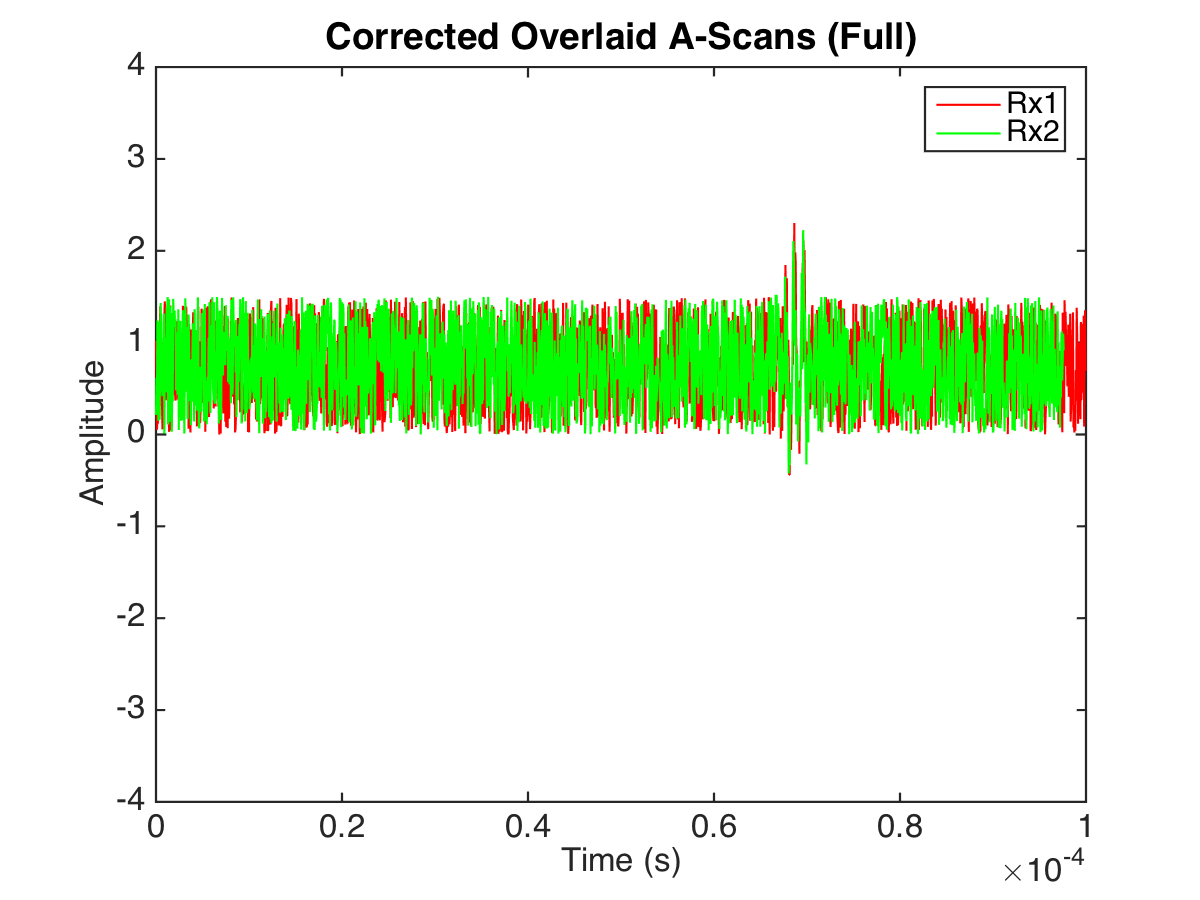
\includegraphics[width=100mm]{Noise_7_Phase.png}
		\caption{Two A-Scans overlaid with added noise and corrected using phase-based CAFI}
		\label{fig:cafi_phase7}
\end{figure}

\begin{figure}[hp]
\centering
		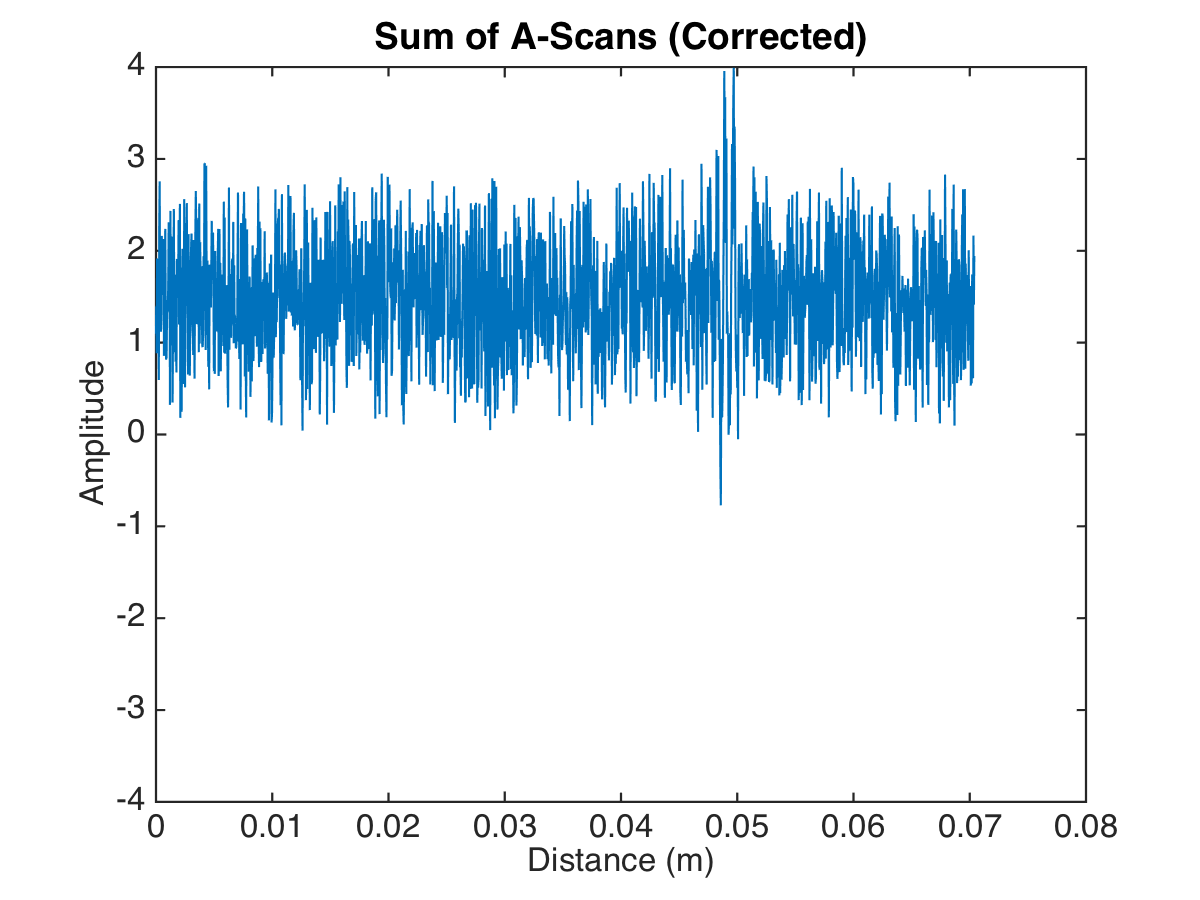
\includegraphics[width=100mm]{Noise_8_Phase.png}
		\caption{Two A-Scans combined with added noise and corrected using phase-based CAFI}
		\label{fig:cafi_phase8}
\end{figure}

The maximum signal value in Figure \ref{fig:cafi_phase8} is 3.8 while the peak noise value is 2.8, meaning that the signal to peak noise ratio is 2.7dB. This is less than the SNR of the amplitude-based CAFI even though the anisotropy has been properly corrected for. The reason for the lower SNR is due to the noise destructively interfering with the reflected signal. 

If more A-Scans were modelled and used to build a new delay-and-sum signal, the phase-based CAFI would eventually outperform the amplitude-based due to the fact that the noise would start to be averaged out and the signals would combine more optimally. 

In some cases both the phase-based and amplitude-based versions of CAFI fail to calculate the correct delays. In these cases, the calculated ideal delays are generally different and will produce different images when each of the delays are used. This can be used to our advantage as the two different generated images can be used as an input to SASACI's cross-correlation algorithm\cite{lardner_new_2013} to attempt to pick out the coherent component of the images.


\subsection{CAFI Imaging}

In previous examples, a model was used with one transmitting and two receiving elements. A Full Matrix Capture dataset can have 64 transmitting elements and 64 receiving elements, though both greater and fewer elements are also commonly used. A slightly different approach is required in order to refine the delays for each A-scan.

For imaging with CAFI, each transmitter and each pixel are treated independently. CAFI will attempt to focus on one pixel for one transmitting element at a time. For an FMC dataset collected from a 64 element array, there will be 64 A-scans to apply the technique to. In the previous examples, there were only 2 A-scans used. It does not matter in these examples if $Rx1$ is correlated with respect to $Rx2$, or the other way around. The ideal delay, if reversed, will simply be the inverse. For multiple A-scans, it does matter which A-scan is correlated with respect to another.

First, the expected delays are calculated for each receiving element using the speed of sound (generally measured with a pulse-echo test on a block of known thickness) within the material. A subset (normally around 300 samples) of each A-scan, centred around where the reflection would be expected (calculated using the estimated velocity), is copied into an array for each receiving element. Each of the A-scans is then correlated with its neighbouring A-scan, always with respect to the element closest to the centre of the array. Once each of the A-scans has been correlated to each other $n-1$ delays will have been calculated, where $n$ is the number of elements in the array.

The delays are then normalised to the centre element (i.e. the centre element has a delay of 0) and the delays are then calculated relative to the centre element. This is done using Equation \ref{eq:cafi_normalise} where $delay$ is the delay to apply to each A-scan, $x$ is the A-scan of interest, $n_{el}$ is the number of array elements and $d_{ci} = d_i - d_c$ is the normalised delay for A-scan, $i$, with respect to its neighbouring element closest to the centre element. If two centre elements exist, $d_c$ is calculated by taking the average of the two.



\begin{equation} \label{eq:cafi_normalise}
delay = \begin{cases}
		\sum\limits_{i = x}^{\frac{n_{el}}{2}} d_{ci}, & \text{if }x<\frac{n}{2}\text{;}\\
		\\
		\sum\limits_{i = \frac{n_{el}}{2}}^{x} d_{ci}, & \text{otherwise.}
\end{cases}
\end{equation}

After these delays have been calculated, standard TFM imaging takes place and a unique delay is calculated for each receive element while looping through each transmitting element and each pixel.

This process can then be repeated with phase-based CAFI in order to generate two different sets of delays and therefore two different images. If this is the case, then two images have been created, each using TFM with a form of focus correction to account for phase aberration. Any legitimate reflectors should be subject to enhanced focusing in the corrected images. Any noise may differ between the two images since most of the noise in a TFM image is from grain reflections that will suffer more from multipath propagation. SASACI cross-correlates images created from the two array sub-apertures to remove grain noise. If two images have been generated then the final stage of the CAFI process is to cross-correlate the focus-corrected images using the two-dimensional cross-correlation algorithm in Equation \ref{eq:XCorr}. Once $p$ is found for each pixel, using this equation, any pixel where $p < 0$ is set to 0. $p$ is then cross-multiplied with the original TFM image to give the final CAFI result.

\section{Results}

CAFI was validated experimentally using an ultrasonically noisy material. Two metrics were used to measure the performance of the technique. The number of pixels with amplitude \textgreater -6 dB are counted. This is an approximate measure of point spread when imaging a small defect. The area within these pixels is determined to be signal and anything outside of this is noise. The mean values of these areas are taken to give the Signal to Noise Ratio (SNR) in dB.

\subsection{Experimental Set-up}

Figure \ref{fig:cafi_setup} shows a block of Inconel 625 which was inspected from the top face with a Vermon 128 element 5MHz linear array driven by a Zetec Dynaray Phased Array Controller. An FMC dataset was captured using a 32 element sub-aperture of the array. The target for inspection is the side drilled hole indicated in Figure \ref{fig:cafi_setup}, which is 60mm from the top surface. 

\begin{figure}[hp]
\centering
		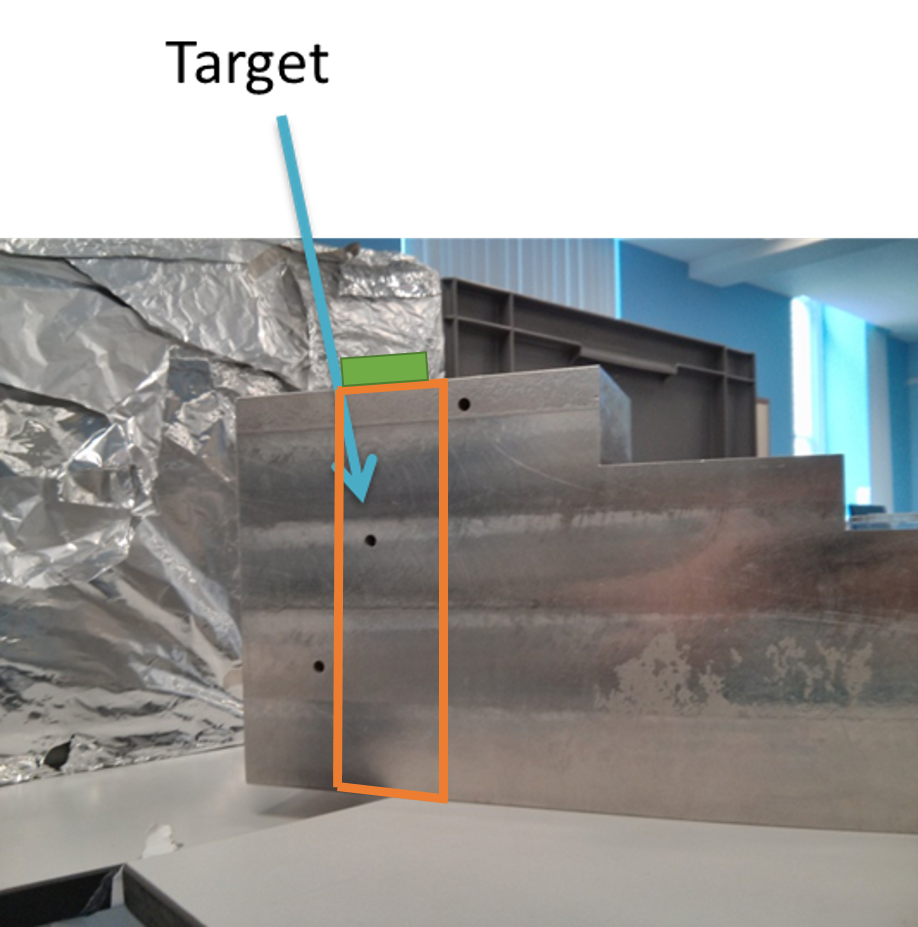
\includegraphics[width=100mm]{setup_2.png}
		\caption{An Inconel 625 step wedge of height 180mm. The area to be imaged is highlighted by an orange box, and the green rectangle represents the array position.}
		\label{fig:cafi_setup}
\end{figure}

The Inconel block is the same specimen used in Section \ref{sec:sasaci_siemens}, however array used to record the data used in this section was positioned at a different point. Due to the internal structure of the material, the velocities and scatterers within the sample change through its cross-section. This gives rise to significantly different results depending on where the array is placed on the sample.

The TFM image of the full depth of the block is shown in Figure \ref{fig:cafi_full_siemens}. The image is shown at a dynamic range of 20dB and has multiple visible defects, one at a depth of 60mm and another at 105mm. Due to the computational complexity of the algorithm (in the order of minutes per pixel), only a small subset of this area will have CAFI applied to it, as depicted by the green rectangle in the image.


\begin{figure}[hp]
\centering
		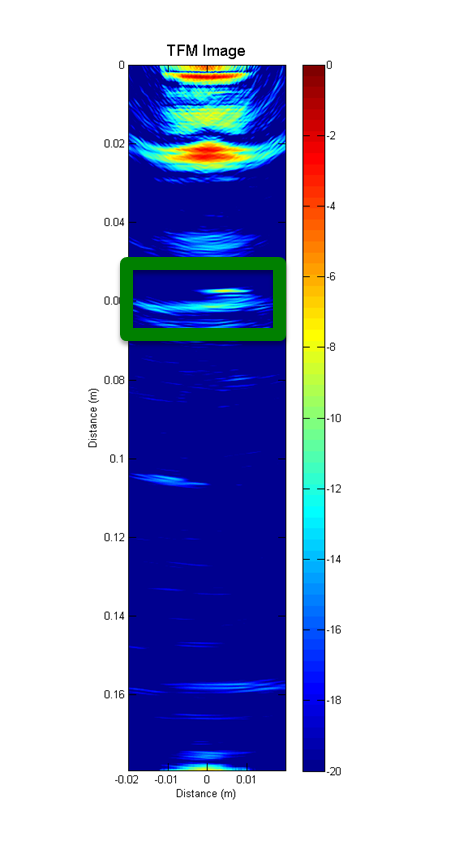
\includegraphics[width=100mm]{full_image.png}
		\caption{A TFM image of the step wedge sample. Reflections from side drilled holes are visible at 60mm and 110mm. The back wall is at 0.16m.}
		\label{fig:cafi_full_siemens}
\end{figure}

\subsection{CAFI Images and Quantitative Results}

Figure \ref{fig:siemens_TFM} shows the TFM image at a dynamic range of 50dB. It has significant contributions of high amplitude noise and the resolution is considered poor. The SNR of this image is 8.16dB and the number of pixels \textgreater -6dB are 179. The main signal is at the correct depth, which is 60mm although it is not clear that there is a side drilled hole in the image. The side drilled hole is clearer in Figure \ref{fig:cafi_full_siemens} due to the 20dB dynamic range in the image. The apparent SNR would also be different due to the size of the area sampled when the noise is measured. This is due to the maximum amplitude within the area shown being normalised to 0dB. Sampling a larger area, where noise would be low due to the lack of reflectors, would result in a lower average noise being measured.

As long as the area where the noise is sampled is the same in each image, a fair comparison can still be drawn between the imaging techniques used. For the following results, all areas in the image \textgreater -6dB are considered signal while the rest are considered noise.

\begin{figure}[hp]
\centering
		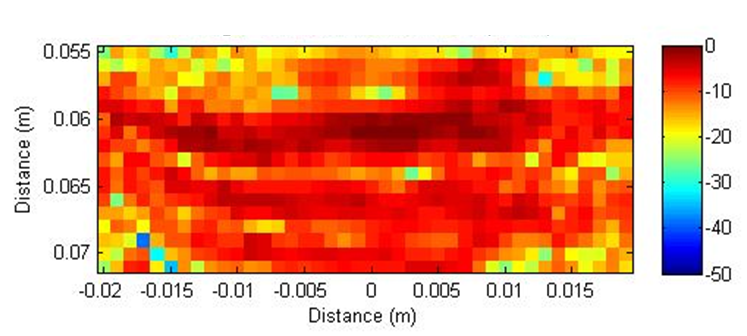
\includegraphics[width=100mm]{siemens_TFM.png}
		\caption{TFM of the side drilled hole}
		\label{fig:siemens_TFM}
\end{figure}

Figure \ref{fig:siemens_CAFI_amp} shows the CAFI image with amplitude-based focus correction. The SNR of this image is 8.59dB which is slightly better than the TFM image. The pixels \textgreater -6dB count is 226 which is poorer than the original TFM image. 

\begin{figure}[hp]
\centering
		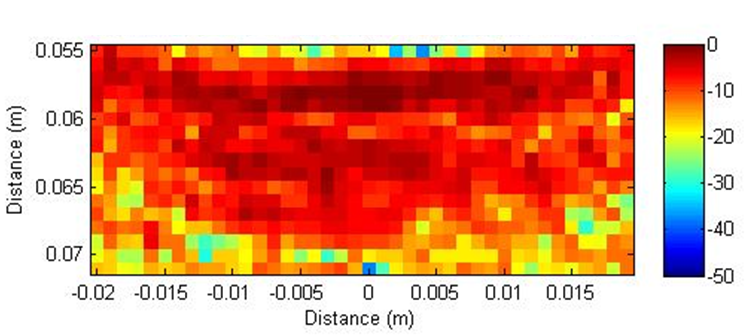
\includegraphics[width=100mm]{siemens_CAFI_amp.png}
		\caption{The side drilled hole with amplitude-based focus correction}
		\label{fig:siemens_CAFI_amp}
\end{figure}

Figure \ref{fig:siemens_CAFI_phase} shows CAFI with phase-based focus correction. The SNR of this image is 7.93dB which is again poorer than the original TFM image but the number of pixels \textgreater -6dB is 164 which represents a slight improvement over TFM. The results from the previous two images show that cross-correlation can be potentially used to improve images due to the differences in both SNR and resolution that can be achieved via standard focus correction algorithms.

\begin{figure}[hp]
\centering
		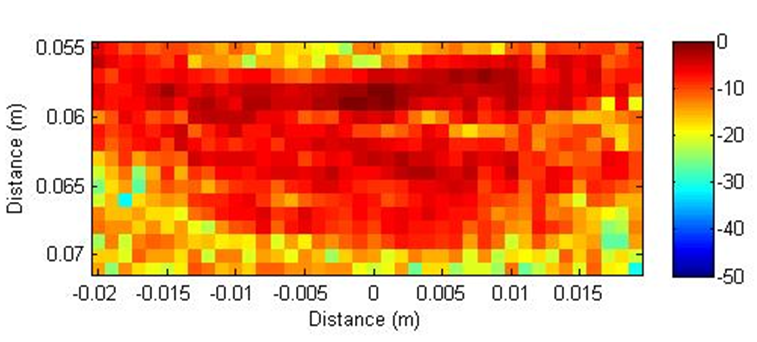
\includegraphics[width=100mm]{siemens_CAFI_phase.png}
		\caption{The side drilled hole with phase-based focus correction}
		\label{fig:siemens_CAFI_phase}
\end{figure}

Figure \ref{fig:siemens_CAFI_SASACI} shows the final CAFI images after the cross-correlation of both the phase-based and amplitude-based corrections. Visually, the hole is present in the image at the expected depth of 60mm, although there are some other artefacts. Quantitatively, the SNR of the image is 36.3dB which is significantly higher than the original TFM image, as well as the intermediary CAFI images. The number of pixels \textgreater -6dB is 6 which shows a large improvement in resolution over TFM.

\begin{figure}[hp]
\centering
		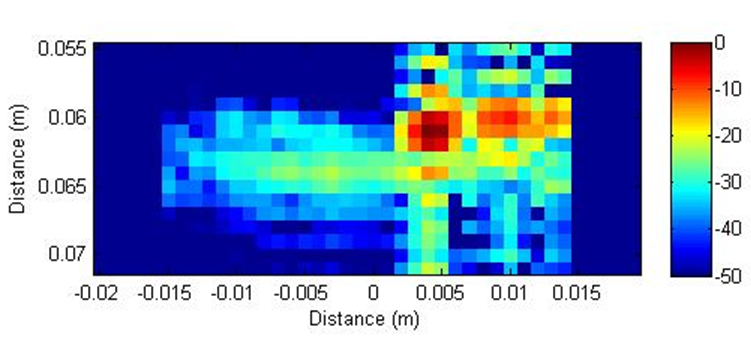
\includegraphics[width=100mm]{siemens_CAFI_SASACI.png}
		\caption{The side drilled hole with the full CAFI method applied}
		\label{fig:siemens_CAFI_SASACI}
\end{figure}


\subsection{Discussion}\label{sec:cafi_discussion}

The Correlation for Adaptively Focused Imaging algorithm was inspired by both Spatially Averaged Sub-Aperture Correlation Imaging and Nearest Neighbour Cross-Correlation. CAFI has a number of advantages over SASACI, including a potential for higher resolution images and robustness to parameter setting which was one of the most significant issues with the practical implementation of SASACI.

The results shown in this chapter show a clear improvement over TFM, although the visible artefacts in the final image demonstrate that the technique still requires improvement.

\begin{table}[ht]
\begin{center}
	\begin{tabular}{| c | c | c |}
	\hline 
	\textbf{Method} & \textbf{SNR} & \textbf{Pixels \textgreater 6dB}\\ \hline \hline 
	TFM	& 8.16dB & 179\\ \hline
	Amplitude-based CAFI & 8.59dB & 226 \\ \hline
	Phase-based CAFI & 7.93dB & 164\\ \hline
	CAFI with SASACI & 36.3dB & 6 \\ \hline
	\end{tabular}
	\caption{Comparison of TFM and different CAFI methodologies}
	\label{table:cafi_results}
	\end{center}
	\end{table}
	
Looking at the quantitative results in Table \ref{table:cafi_results}, it can be seen that the phase-based CAFI and amplitude-based CAFI have different values of SNR and point spread. This is expected due to the fact that the material has large grains which contribute to coherent noise. This coherent noise will affect the outcome of the cross-correlation function and hinder the identification of a defect. As discussed in the methodology section, combining SASACI and CAFI has the potential to create images superior to standard CAFI and this is demonstrated in both the table and in Figure \ref{fig:siemens_CAFI_SASACI}.

A limitation of CAFI is that when there is no defect to focus upon, the cross-correlation function can end up choosing delays where reflections from the grain will sum constructively and appear similar to a genuine defect. For this reason, when CAFI is applied to a large area, the SNR can be comparatively low compared with TFM. It is therefore recommended that CAFI is used to characterise, instead of to determine the location of defects. It is here that CAFI excels and this can be seen when comparing TFM in Figure \ref{fig:siemens_TFM} with the full CAFI method in Figure \ref{fig:siemens_CAFI_SASACI}.

CAFI also has a technical drawback, which is its computational complexity, resulting in significant time required to process images. This can be alleviated by utilizing parallel computing. CUDA based imaging has been discussed in Chapter \ref{chap:cuetfm} and this technique of accelerating the imaging process can also be applied to CAFI as each `loop' of the algorithm is independent from the last.




% ------------------------------------------------------------------------


%%% Local Variables: 
%%% mode: latex
%%% TeX-master: "../thesis"
%%% End: 
